\chapter{Processi gaussiani}\label{gaussianProcessChapter}
In questo capitono vengono introdotti i \textbf{processi gaussiani}. Inevitabilmente il capitolo non sarà esaustivo dell'argomento ma saranno trattate le sue caratteristiche principali e interessanti ai fini dell'elaborato. Per questo motivo la trattazione non si dedicherà ad inquadrare i processi gaussiani nel vasto contesto dei processi stocastici e si limiterà ad uno studio mirato delle sue peculiarità.\\
I codici python usati nel capitolo richiedono di eseguire i codici \ref{import} e \ref{import2} di import delle librerie. Inoltre la media cubica viene per tutti i kernel definita come nel codice \ref{cubedMean}. 
Il codice per le immagini dei kernel si ispira a quello scritto da Peter Roelants nel suo blog alla pagina "\href{https://peterroelants.github.io/posts/gaussian-process-tutorial/#Gaussian-processes-(1/3)---From-scratch}{Gaussian processes - From scratch}". Sono state fatte importanti modifiche al codice, in particolare vengono usati i kernel implementati dalla libreria scikit-learn.
Il codice per la predizione di dati prende invece spunto dal sito  \href{https://docs.w3cub.com/about/}{W3cubDocs} alla pagina "\href{https://docs.w3cub.com/scikit_learn/auto_examples/gaussian_process/plot_gpr_noisy_targets}{Gaussian Processes regression: basic introductory example}". Anche in questo caso sono state fatte importanti modifiche nel codice.
Il codice sulla concentrazione di $CO_2$ è una modifica del codice "\href{https://scikit-learn.org/stable/auto_examples/gaussian_process/plot_gpr_co2.html}{Gaussian process regression (GPR) on Mauna Loa CO2 data}" presente nella documentazione di scikit-learn.\\
Le fonti usate per la stesura del capitolo sono: \cite{rasmussen_gaussian_2006}, \cite{murphy_probabilistic_2022}, \cite{rasmussen_gaussian_2004}, \cite{duvenaud_automatic_2014}, \cite{gortler_visual_2019}, \cite{murphy_machine_2012}.


\begin{textblock*}{0.64\textwidth}(3.5cm+0.36\textwidth,18.5cm)
\epigraph{In applying mathematics to subjects such as physics
or statistics we make tentative assumptions about the
real world which we know are false but which we believe
may be useful nonetheless. The physicist knows that
particles have mass and yet certain results, approximating
what really happens, may be derived from the assuhption that they do not. Equally, the statistician knows, for
example, that in nature there never was a normal distribution, there never was a straight line, yet with normal and
linear assumptions, known to be false, he can often derive
results which match, to a useful approximation, those
found in the real world.}{George E. P. Box}
\end{textblock*}

\newpage


%%%%%%%%%%%%%%%%%%%%%%%%%%%%%%
%%%%% DEFINIZIONE
%%%%%%%%%%%%%%%%%%%%%%%%%%%%%%
\section{Definizione e motivazione}


\begin{defi}[Processo gaussiano]
Un \textbf{processo gaussiano} è un insieme di variabili casuali tali che ogni suo sottoinsieme finito abbia distribuzione gaussiana multivariata.
\end{defi}

Dalla definizione risulta evidente come la teoria delle distribuzioni gaussiane multivariate abbia notevole importanza nello studio dei processi gaussiani.\\
Similmente alla distribuzione gaussiana, completamente determinata dal suo vettore media e dalla sua matrice di covarianza,  i processi gaussiani sono completamente determinati da una \textit{mean function} (che ne determina la media), denotata $m(x)$, e da una \textit{covariance function} (che ne determina la covarianza), denotata $k(x,x')$. Verrà approfondito il ruolo delle due funzioni nella prossima sezione.\\
Nonostante questa similarità però, le distribuzioni gaussiane e i processi gaussiani differiscono per una importante caratteristica: le prime lavorano con vettori, i secondi con funzioni.

\vspace{0.5cm}

\begin{oss}[Motivazione: regressione nonlineare]
La principale applicazione dei processi gaussiani, nonché il tema principale di questo capitolo, è quello della \textbf{regressione nonlineare}.\\
Mentre il modello di regressione lineare cerca, a partire da dati osservati, una relazione lineare tra una variabile dipendente $Y$ e una variabile indipendente $x$, tenendo conto di un errore statistico $\epsilon$, in forma: $Y_i=\beta_0+\beta_1 x_i+\epsilon_i$, dove le incognite sono $\beta_0$ e $\beta_1$; la regressione nonlineare è una forma di regressione in cui la funzione che esprime la relazione tra variabili indipendenti e dipendenti è una combinazione non lineare dei parametri del modello e dipende da una o più variabili indipendenti, dunque in forma: $Y=f(X,\theta)+\epsilon$, dove le incognite sono $\theta$ e la funzione $f$.\\
Una importante differenza tra i due tipi di regressione è che per quella nonlineare, a differenza di quella lineare, non esiste un metodo generale per la determinazione dei valori dei parametri. 

%%%%%%%%%%%%%%%%%%%%%%%%%%%%%%%%%%%
%%%%%% IMMAGINE REGRESSIONE NONLINEARE
%%%%%%%%%%%%%%%%%%%%%%%%%%%%%%%%%%%
\begin{figure}[h]
\centering
\begin{subfigure}{.5\textwidth}
  \centering
  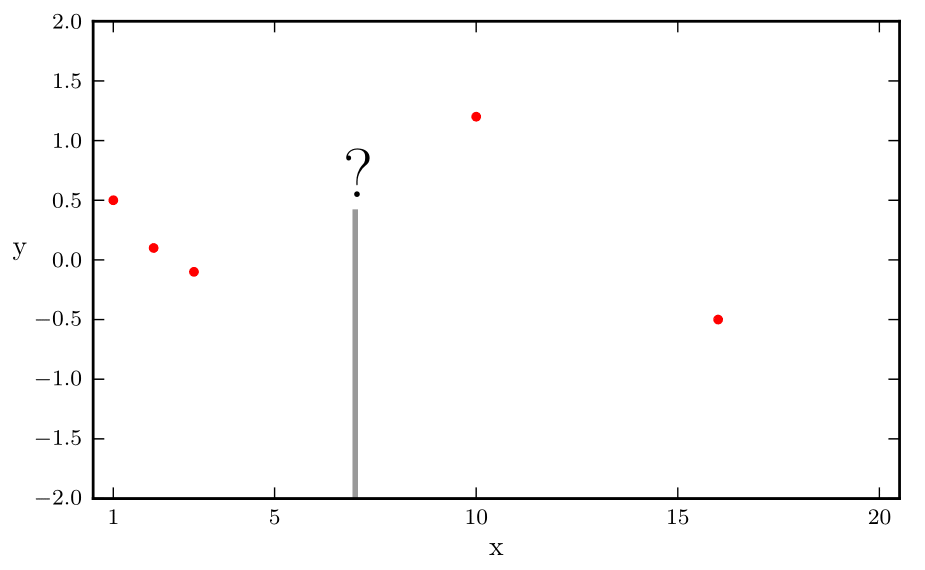
\includegraphics[width=\linewidth]{images/Gaussian process/motivazione2.png}
\end{subfigure}%
\begin{subfigure}{.5\textwidth}
  \centering
  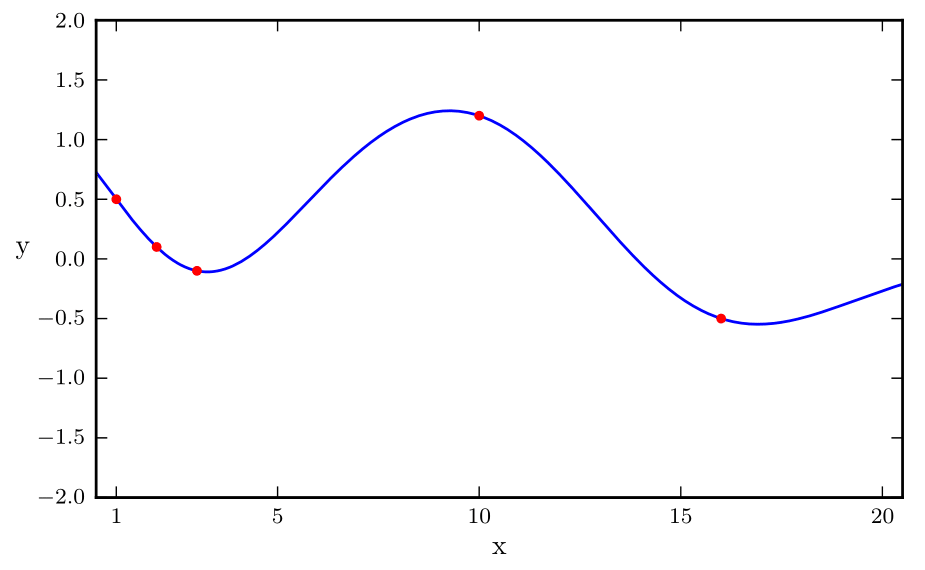
\includegraphics[width=\linewidth]{images/Gaussian process/motivazione3.png}
\end{subfigure}
\caption{Regressione nonlineare \cite{turner_gaussian_2016}.}
\end{figure}


\newpage

I \textbf{processi gaussiani} forniscono un buon metodo per la determinazione dei parametri nella regressione nonlineare non solo perché sfruttano la teoria della distribuzione gaussiana multivariata, complessivamente semplice, ma perché oltre ad una funzione che  approssima i dati in modo nonlineare con massima probabilità (concetto chiarito successivamente) forniscono un'indicazione della confidenza della regressione in forma di un'area all'interno della quale funzioni interpolanti meno probabili (ma comunque possibili) risiedono, come illustrato in figura \ref{nonlinearRegressionGaussianProcess}.


%%%%%%%%%%%%%%%%%%%%%%%%%%%%%%%%%%%
%%%%%% IMMAGINE REGRESSIONE NONLINEARE GAUSSIANA
%%%%%%%%%%%%%%%%%%%%%%%%%%%%%%%%%%%
\begin{figure}[h]
    \centering
    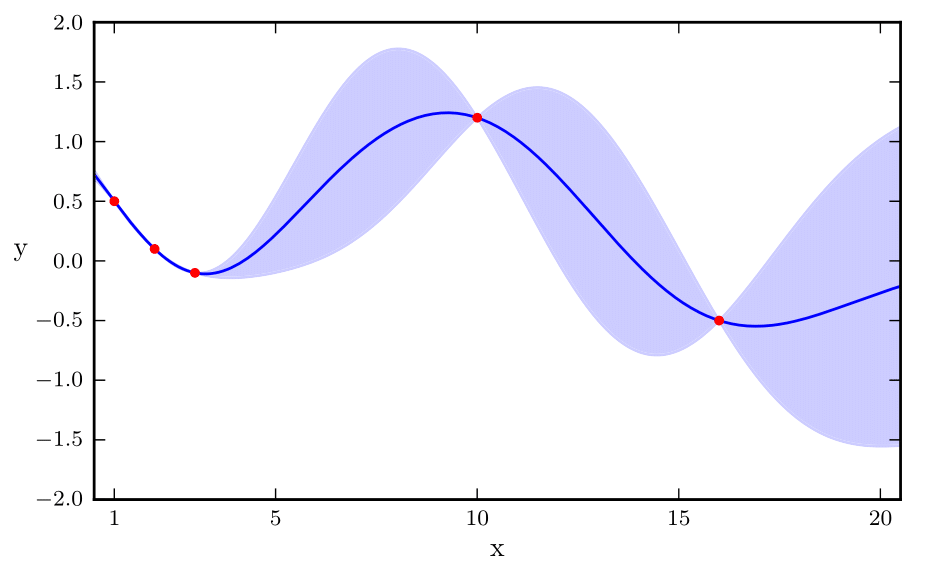
\includegraphics[width=0.85\textwidth]{images/Gaussian process/motivazione4.png}
    \caption{Regressione nonlineare con processi gaussiani \cite{turner_gaussian_2016}.}
    \label{nonlinearRegressionGaussianProcess}
\end{figure}

\end{oss}

\newpage

\section{Introduzione ai processi gaussiani e alla notazione}
Seppur non rientri negli scopi dell'elaborato approfondire questo aspetto, viene riportata la definizione di processo stocastico per facilitare l'introduzione della notazione usata.



%%%%%%%%%%%%%%%%%%%%%%%%%%%%
%%%%%% PROCESSO STOCASTICO
%%%%%%%%%%%%%%%%%%%%%%%%%%%%
\begin{defi}[Processo stocastico]
Un \textbf{processo stocastico} su uno spazio di probabilità $(\Omega, \mathcal{F}, \mathbb{P})$ è una famiglia $\{X_t\}_{t\in T\subset \mathbb{R}}$ di variabili casuali indicizzata da un parametro $t$.
\end{defi}



È comune chiamare $t$ l'indice per sottolineare il ruolo del tempo nei processi stocastici: un processo stocastico, generalmente, descrive matematicamente l'evoluzione temporale di un sistema caratterizzato dall'essere soggetto al caso, un sistema, cioè, del quale lo stato al tempo $t$ non può essere determinato con certezza ma solo da una variabile casuale.\\
In un sistema stocastico è dunque possibile solo calcolare la \textit{probabilità} che il sistema si trovi in uno degli stati possibili ad un tempo $t>t_0$ se è noto lo stato al tempo $t_0$; in un sistema deterministico invece l'evoluzione viene descritta da regole (tipicamente in forma di equazione differenziale) che consentono di determinare con precisione lo stato del sistema ad ogni tempo $t>t_0$ noto lo stato al tempo $t_0$.




%%%%%%%%%%%%%%%%%%%%%%%%%
%%%%%%% NOTAZIONE
%%%%%%%%%%%%%%%%%%%%%%%%%
\begin{nota}[Funzioni e indicizzazione nei processi gaussiani]
Scrivendo $f\sim \mathcal{GP}(m,k)$ si  intende che "\textit{la funzione $f$ è distribuita come un processo gaussiano con mean function $m(\cdot)$ e covariance function $k(\cdot,\cdot)$}".\\
La funzione così ottenuta si può descrivere come:
\[f: \chi \rightarrow \mathbb{R},\]
dove $\chi$ è un qualsiasi dominio. Per ogni elemento $x$ nel dominio $\chi$ esiste una variabile casuale $f(x)$ a cui è associato.
\end{nota}



\begin{oss}[Versatilità dei processi gaussiani e generalizzazione dei vettori gaussiani] \label{oss1}
Si noti che il dominio $\chi$ non ha restrizioni, caratteristica che rende i processi gaussiani molto versatili. Si noti inoltre che con un dominio finito un processo gaussiano è un vettore gaussiano multivariato. In questo senso, come detto in precedenza, i processi gaussiani sono una generalizzazione dei vettori gaussiani multivariati. 
\end{oss}


\newpage
%%%%%%%%%%%%%%%%%%%%%
%%%%%% MEAN FUNCTION
%%%%%%%%%%%%%%%%%%%%%
\begin{defi}[Mean function]
Dato un processo gaussiano $f\sim \mathcal{GP}(m,k)$, la \textbf{mean function} è una funzione
\[
m:\chi \rightarrow \mathbb{R}
\]
dove $m(x)=\mathbb{E}[f(x)]$.
\end{defi}

\begin{oss}
Per la \textit{mean function} non vi è alcuna richiesta in termini di proprietà della funzione. Tipiche scelte sono $m(x)=0$ oppure $m(x)=c$ con $c$ costante.
\end{oss}

Diversamente dalla \textit{mean function}, la scelta della \textit{covariance function} è ristretta a una determinata classe di funzioni, perciò prima della definizione vengono introdotti alcuni concetti preliminari.




%%%%%%%%%%%%%%%%%%%%%%%%
%%%% MERCER KERNEL
%%%%%%%%%%%%%%%%%%%%%%%%
\begin{defi}[Mercer kernel/positive definite kernel]
Si definisce \textbf{Mercer kernel} (o \textbf{positive definite kernel}) qualunque funzione simmetrica 
\[
\mathcal{K}: \chi\times\chi \rightarrow \mathbb{R}^+
\]
 tale che: $\sum_{i=1}^N\sum_{j=1}^N\mathcal{K}(x_i,x_j)c_ic_j \geq 0$ per qualunque insieme di elementi distinti $\{x_i\}_{i=1}^N\subset \chi$, $\{c_i\}_{i=1}^N\subset  \mathbb{R}$.
\end{defi}

Una definizione alternativa si basa sul concetto di \textit{matrice di Gram}:

\begin{defi}[Matrice di Gram]
Data una funzione $\mathcal{K}: \chi\times \chi\rightarrow \mathbb{R}^+$, sia $\{x_i\}_{i=1}^N\subset \chi$ un insieme qualsiasi di elementi distinti, si definisce la \textbf{matrice di Gram} di $\mathcal{K}$ la seguente:
\[
\bm{K}=\begin{pmatrix}
    \mathcal{K}(x_1,x_1) & \mathcal{K}(x_1,x_2) & \dots & \mathcal{K}(x_1,x_N)\\
    \mathcal{K}(x_2,x_1) & \mathcal{K}(x_2,x_2) & \dots & \mathcal{K}(x_2,x_N)\\
    \vdots & \vdots & \ddots & \vdots\\
    \mathcal{K}(x_N,x_1) & \mathcal{K}(x_N,x_2) & \dots & \mathcal{K}(x_N,x_N)
    \end{pmatrix}
\]
\end{defi}

\begin{defi}[Mercer kernel/positive definite kernel]
Data una funzione $
\mathcal{K}: \chi\times\chi \rightarrow \mathbb{R}^+
$, $\mathcal{K}$ si dice \textbf{Mercer kernel} se e solo se la sua matrice di Gram è semidefinita positiva.
\end{defi}

È ora possibile definire la covariance function.

\newpage


%%%%%%%%%%%%%%%%%%%%%%%%
%%%% COVARIANCE FUNCTION
%%%%%%%%%%%%%%%%%%%%%%%%
\begin{defi}[Covariance/kernel function]
Dato un processo gaussiano $f\sim \mathcal{GP}(m,k)$, la \textbf{covariance function} è una funzione
\[
k:\chi\times \chi \rightarrow \mathbb{R}
\]
tale che $k(\cdot,\cdot)$ è un \textit{Mercer kernel}. Si ha 
\[k(x,x')=\mathbb{E}[(f(x)-m(x))(f(x')-m(x'))]=\text{Cov}[f(x),f(x')].
\]
\end{defi}

\begin{oss}[Similarità tra processi gaussiani e distribuzione gaussiana multivariata]
Si è definita la \textit{mean function} senza fare restrizioni sulle proprietà della funzione mentre per la \textit{covariance function} è stato richiesto che la sua matrice di Gram sia semidefinita positiva.\\
Questo non deve sorprendere: come precedentemente detto, i processi gaussiani generalizzano la distribuzione gaussiana multivariata e come spiegato nel precedente capitolo (e enfatizzato nell'osservazione \ref{ossGaussianaMultivariata}) quest'ultima è definita da due parametri: un vettore media, senza alcuna restrizione, e una matrice di covarianza, che deve essere simmetrica e  semidefinita positiva. Vi è dunque, anche in questo senso, similarità tra processi gaussiani e distribuzioni gaussiane multivariate.
\end{oss}

\vspace{0.5cm}

%%%%%%%%%%%%%%%%%%%%%%%%%%%%
%%%%%%% ESEMPIO GP
%%%%%%%%%%%%%%%%%%%%%%%%%%%
\begin{ese}[Esempio di processo gaussiano] \label{esempioProcessoGaussiano}
Si consideri $f\sim \mathcal{GP}(m,k)$, dove:
\[
m(x)=\frac{x^2}{4}\qquad k(x,x')=\text{exp}\left( -\frac{1}{2}(x-x')^2\right).
\]
Per comprendere questo esempio di processo gaussiano si consideri il grafico di alcuni campioni della funzione $f$. Per non lavorare nel caso infinito, si consideri un dominio finito\footnote{Si tenga conto che dal punto di vista teorico i processi gaussiani che vengono considerati in questo elaborato si costruiscono su un dominio infinito di numeri reali; tuttavia quando si generano i grafici si è costretti a considerare un insieme finito di punti che poi vengono uniti per generare la curva. Con questa (obbligata) filosofia vengono costruiti i grafici della prossima sezione.\label{footnote 1}}: $\chi = \left\{x_i \right\}_{i=1}^{n}$. Essendo $\chi$ finito, quello che si ottiene valutando $m(\cdot)$ e $k(\cdot,\cdot)$ sul dominio sono un vettore $\bm{\mu}$ e una matrice $\bm{\Sigma}$ dove:
\[
\begin{split}
\mu_i&=m(x_i)=\frac{x_i^2}{4} \qquad\qquad\qquad\qquad\qquad\qquad i=1,\dots, n \\
\Sigma_{ij}&=k(x_i,x_j)=\text{exp}\left( -\frac{1}{2}(x_i-x_j)^2\right)\qquad i,j=1,\dots, n
\end{split}
\]
Si ottiene quindi, come anticipato nell'osservazione \ref{oss1}, che per ogni $x_i$ nel dominio $\chi$ la variabile casuale $f(x_i)$ è un variabile casuale gaussiana di media $\mu_i$ e varianza $\Sigma_{ii}$; chiamando $\bm{f}=(f(x_1), \dots, f(x_n))^{\text{T}}$ si ha cioè: 
\[
\bm{f}\sim \mathcal{N}(\bm{\mu}, \bm{\Sigma}).
\]

\newpage

 Avendo ottenuto un vettore gaussiano multivariato $n$-dimensionale risulta naturale utilizzare lo stesso metodo introdotto nella sezione \ref{sezioneCorrelazione} per ricavare il grafico della "funzione" (è in realtà un vettore) $\bm{f}$. Nella figura \ref{esempioProcessoGaussianoImmagine} vengono riportati i "grafici" di quattro campioni diversi di vettore gaussiano di dimensione $n=60$. Si noti che la forma dei quattro grafici è ben diversa da quella della figura \ref{correlazione6} come conseguenza del fatto che le distribuzioni hanno matrice di covarianza diversa. Questo sottolinea quanto sia importante la covariance function nei processi gaussiani, essendo responsabile della matrice di covarianza. Questo argomento verrà analizzato in dettaglio successivamente.\newline
 Con questo esempio si è chiarito cosa si intende quando si è detto che i processi gaussiani generalizzano la distribuzione gaussiana multivariata.

%%%%%%%%%%%%%%%%%%%%%%%%%
%%%%%%%%% IMMAGINE
%%%%%%%%%%%%%%%%%%%%%%%%
\begin{figure}[h]
    \centering
    \includegraphics[width=0.85\textwidth]{images/Gaussian process/esempioProcessoGaussiano.pdf}
    \caption{Quattro vettori generati da un processo gaussiano definito come  nell'esempio \ref{esempioProcessoGaussiano}. Codice \ref{Example}.}
    \label{esempioProcessoGaussianoImmagine}
\end{figure}

Si noti che il codice \ref{Example} non genererà lo stesso grafico della figura \ref{esempioProcessoGaussianoImmagine} in quanto c'è una componente randomica! Lo stesso vale per gli altri codici citati in questo capitolo.
\end{ese}


\newpage


%%%%%%%%%%%%%%%%%%%%%%%%%%
%%%%% SULLE COVARIANCE FUNCTION
%%%%%%%%%%%%%%%%%%%%%%%%%%


\section{Sulle covariance function}
Per un processo gaussiano è di fondamentale importanza la covariance function: è infatti la funzione $k(\cdot,\cdot)$ che determina come il processo gaussiano interpreta i dati: a partire dalla definizione della covariance function è possibile ricavare diversi modelli, ad esempio la regressione lineare \footnote{Per approfondire si veda \cite{rasmussen_gaussian_2006}  e  \cite{williams_prediction_1998}} o le splines \footnote{Per approfondire si veda \cite{kimeldorf_correspondence_1970}}.\\
\begin{oss}[Importanza della covarianza]
Nel precedente capitolo, alla sezione \ref{sezioneCorrelazione}, è stata mostrata un'interpretazione visiva dell'indice di correlazione di Pearson ed è stato  chiarito come la covarianza influisca sulla correlazione di due variabili casuali.\\
Risulta quindi evidente l'importanza della covariance function nella correlazione tra le variabili casuali $f(x)$ e $f(x')$ per ogni $x,x'\in \chi$. Per questo motivo è significativo, nella scelta della covariance function, tenere conto di come questa dipenda dalla coppia $(x,x')$.
\end{oss}

Seguono i tre principali tipi di covariance function in base alla loro dipendenza da $(x,x')$ dove $x,x'\in \mathbb{R}^D$.




%%%%%%%%%%%%%%%%%%%%%%%%%%
%%%%%%% PROPRIETA KERNEL
%%%%%%%%%%%%%%%%%%%%%%%%%%
\begin{defi}[Covariance function stazionaria]
Una covariance function \textbf{stazionaria} è una covariance function che dipende da $x-x'$.\\
Una covariance function di questo tipo è invariante per traslazioni.
\end{defi}

\begin{defi}[Covariance function isotropica]
Una covariance function \textbf{isotropica} è una covariance function che dipende da $||x-x'||$.\\
Una covariance function di questo tipo è invariante per movimenti rigidi.
\end{defi}

\begin{defi}[Dot product covariance function]
Una \textbf{dot product} covariance function è una covariance function che dipende da $x$ e $x'$ solo tramite $x\cdot x'$.\\
Una covariance function di questo tipo è invariante per rotazioni centrate nell'origine ma non per traslazioni.
\end{defi}

Di seguito vengono mostrate le principali covariance function. Come già detto in precedenza, questa non può che essere un'introduzione alle possibili scelte: importanti aspetti delle covariance function riguardano la loro generalizzazione data dall'uso della distanza di Mahalanobis, una corretta scelta del kernel per l'ottimizzazione numerica, relazione tra scelta del kernel e deep learning per i processi gaussiani \footnote{Per approfondire si veda \cite{murphy_probabilistic_2022}}, adattamento dei kernel a modelli a più dimensioni \footnote{Per approfondire si veda \cite{duvenaud_automatic_2014}}... \\
In merito alle covariance function, è negli interessi di questo elaborato comprendere come queste influiscano nel processo gaussiano. Insieme ai prossimi esempi verranno quindi riportati dei grafici a supporto di questo interesse.

\newpage

\subsection{Linear kernel}
%%%%%%%%%%%%%%%%%%%%%%%%%
%%%% LINEAR
%%%%%%%%%%%%%%%%%%%%%%%
\begin{defi}[Linear kernel]
Il \textbf{linear kernel} ha forma \[
k(x,x')=\sigma_b^2+\sigma_v^2 (x-c)(x'-c).
\]
\end{defi}

Viene riportato il grafico della funzione $k(x,x')$. Si ottiene una retta con gli usuali parametri.
%%%%%%%%%%%%%%%%%%%%%%%%%
%%%%%%%%% IMMAGINE
%%%%%%%%%%%%%%%%%%%%%%%%
\begin{figure}[h]
    \centering
    \includegraphics[width=0.6\textwidth]{images/Gaussian process/Linear Kernel.pdf}
    \caption{Grafico di $k(x,x')$ linear kernel, $\sigma_b^2=1$, $\sigma_v^2=1$, $c=-1$ e $x'=1$. Codice \ref{linear kernel code}}
    \label{linear kernel}
\end{figure}

\newpage

Nella figura \ref{10 sample linear kernel zero mean} vengono mostrati grafici di funzioni con distribuzione $f\sim \mathcal{GP}(m,k)$ dove $m(x)=0$ e $k(x,x')$ è il linear kernel, $\sigma_b^2=0$, $\sigma_v^2=1$, $c=0$.



%%%%%%%%%%%%%%%%%%%%%%%%%%%%
%%%%%%%% IMMAGINE
%%%%%%%%%%%%%%%%%%%%%%%%%%%
\begin{figure}[h]
    \centering
    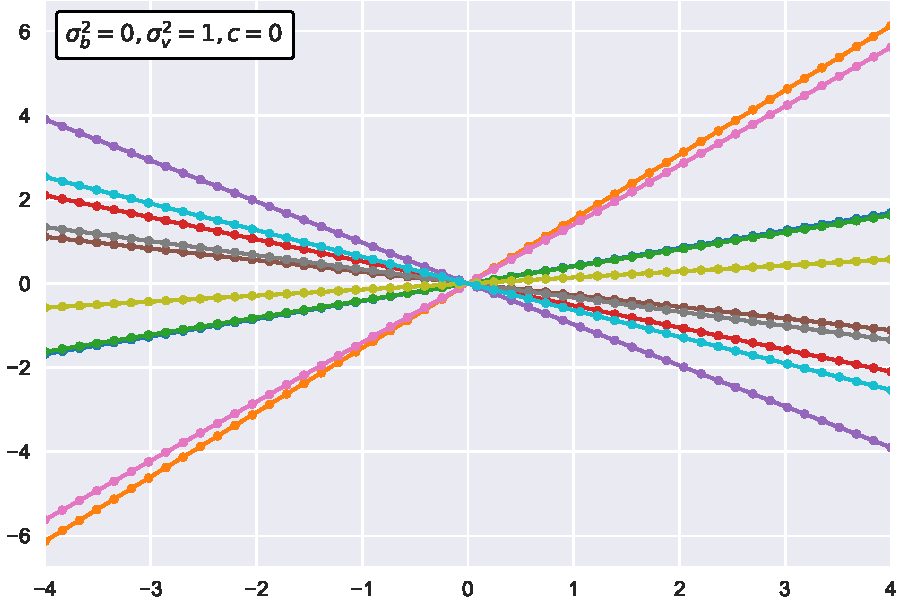
\includegraphics[width=0.85\textwidth]{images/Gaussian process/Linear sample.pdf}
    \caption{Grafico di funzioni con distribuzione  $f\sim \mathcal{GP}(\bm{0},k)$ dove $k(x,x')$ è il linear kernel e $\sigma_b^2=0$, $\sigma_v^2=1$, $c=0$. Codice \ref{linear sample}.}
    \label{10 sample linear kernel zero mean}
\end{figure}

Si noti che il linear kernel genera delle rette, da cui il nome.\\
Imporre la mean function uguale a zero aumenta la tendenza delle linee a passare per l'origine. Imponendo $m(x)=\alpha\in\mathbb{R}$ si aumenta la tendenza delle rette a passare per il punto $(0,\alpha)$. 
%Esploreremo di seguito l'influenza degli altri parametri del kernel sui grafici delle funzioni, ma è già in parte evidente l'importanza della struttura del kernel nel grafico delle funzioni con distribuzione $\mathcal{GP}(m,k)$.



\newpage






\vspace{1cm}
Per comprendere l'influenza del parametro $c$, vengono mostrati grafici di funzioni con distribuzione $f\sim \mathcal{GP}(m,k)$ dove $m(x)=0$ e $k(x,x')$ è il linear kernel e viene variato il valore di $c$.

%%%%%%%%%%%%%%%%%%%%%%%%%%%%%%%%%%%
%%%%%% IMMAGINI: PARAMETRO c
%%%%%%%%%%%%%%%%%%%%%%%%%%%%%%%%%%%
\begin{figure}[h]
\centering
\begin{subfigure}{.5\textwidth}
  \centering
  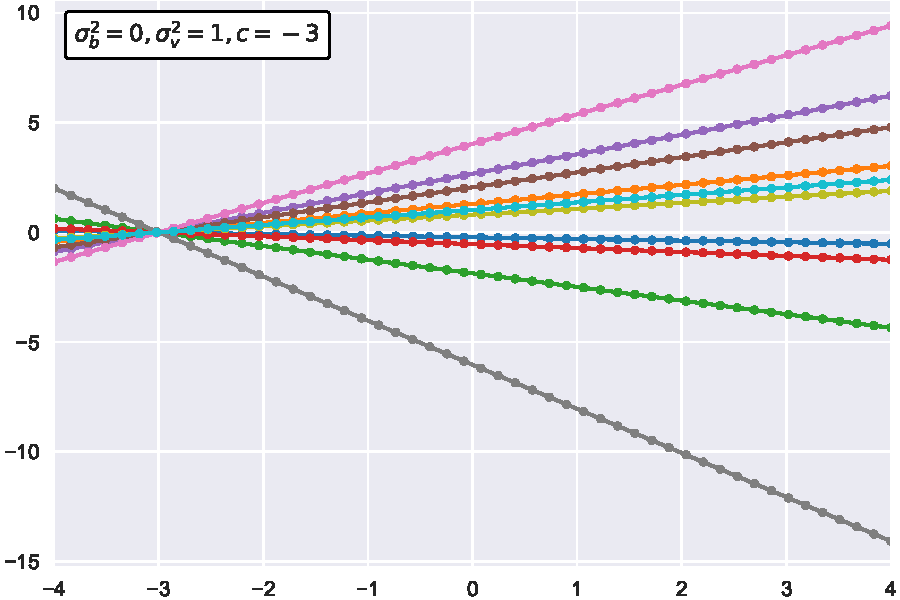
\includegraphics[width=\linewidth]{images/Gaussian process/Linear - c=-3.pdf}
  \caption{$c=-3$}
\end{subfigure}%
\begin{subfigure}{.5\textwidth}
  \centering
  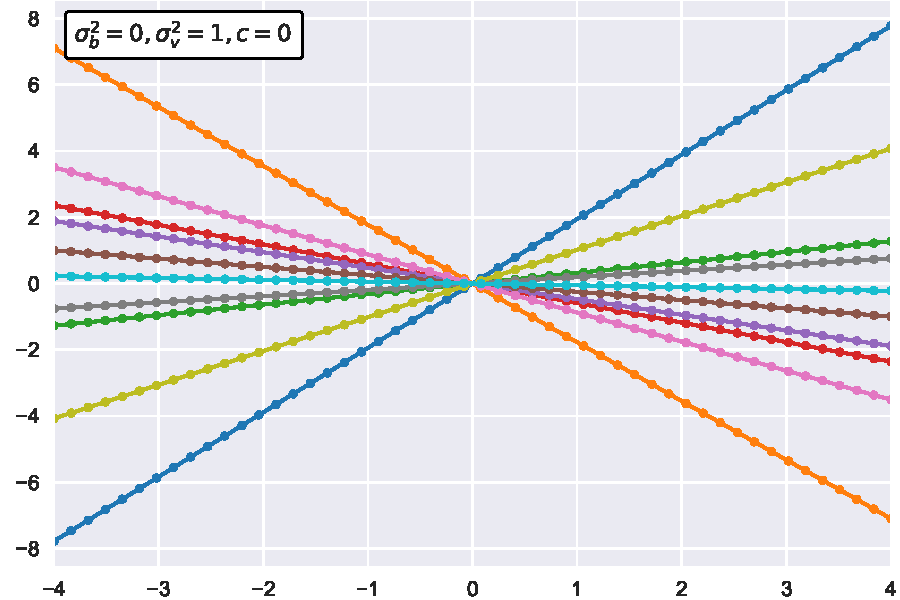
\includegraphics[width=\linewidth]{images/Gaussian process/Linear - c=0.pdf}
  \caption{$c=0$}
\end{subfigure}
\caption{Grafico di funzioni con distribuzione $f\sim \mathcal{GP}(\bm{0},k)$ dove $k(x,x')$ è il linear kernel e $\sigma_b^2=0$, $\sigma_v^2=1$, il parametro $c$ viene variato. Codice \ref{Linear - c}.}
\label{10 sample linear modified c}
\end{figure}


Il parametro $c$ dunque impone un punto di passaggio per tutte le rette. Dunque $c$ svolge lo stesso ruolo della mean function $m(\cdot)$.

Per comprendere l'influenza del parametro $\sigma_b^2$, vengono mostrati grafici di funzioni con distribuzione $f\sim \mathcal{GP}(m,k)$ dove $m(x)=0$ e $k(x,x')$ è il linear kernel e viene variato il valore di $\sigma_b^2$.

%%%%%%%%%%%%%%%%%%%%%%%%%%%%%%%%%%%
%%%%%% IMMAGINI: PARAMETRO sigma_b
%%%%%%%%%%%%%%%%%%%%%%%%%%%%%%%%%%%
\begin{figure}[h]
\centering
\begin{subfigure}{.5\textwidth}
  \centering
  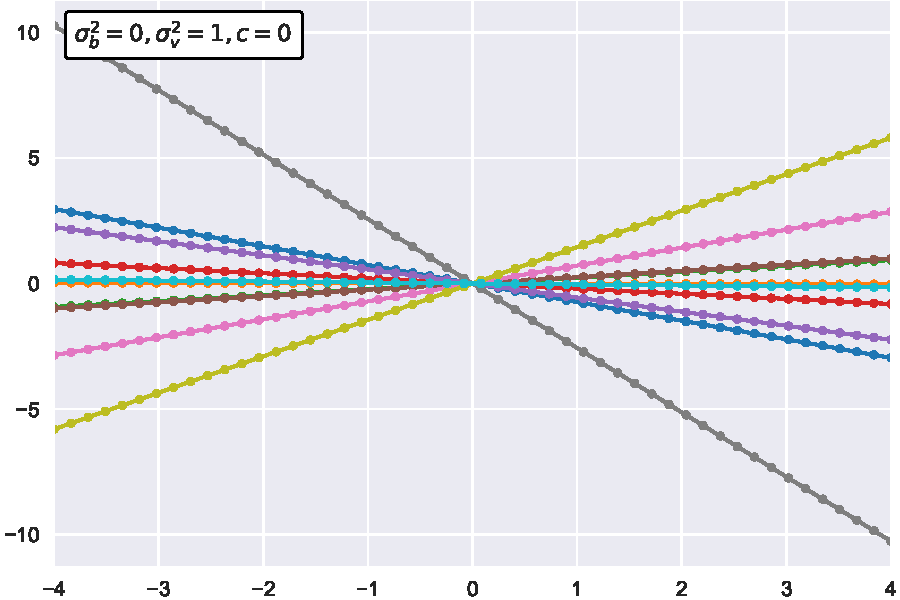
\includegraphics[width=\linewidth]{images/Gaussian process/Linear - sigmab=0.pdf}
  \caption{$\sigma_b^2=0$}
\end{subfigure}%
\begin{subfigure}{.5\textwidth}
  \centering
  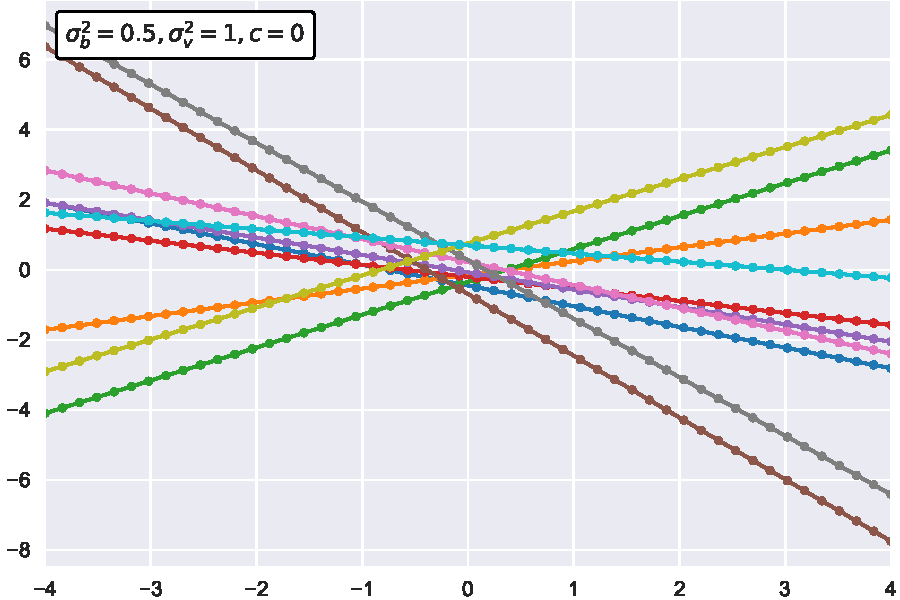
\includegraphics[width=\linewidth]{images/Gaussian process/Linear - sigmab=05.pdf}
  \caption{$\sigma_b^2=0.5$}
\end{subfigure}
\caption{Grafico di funzioni con distribuzione $f\sim \mathcal{GP}(\bm{0},k)$ dove $k(x,x')$ è il linear kernel e $\sigma_v^2=1$, $c=0$, il parametro $\sigma_b^2$ viene variato. Codice \ref{Linear - sigmab}.}
\label{10 sample linear modified sigmab}
\end{figure}
Dunque il parametro $\sigma_b$ influenza la precisione con cui le funzioni tendono a passare per il punto $(0,c)$.

\newpage

Per comprendere l'influenza del parametro $\sigma_v^2$, vengono mostrati grafici di funzioni con distribuzione $f\sim \mathcal{GP}(m,k)$ dove $m(x)=0$ e $k(x,x')$ è il linear kernel e viene variato il valore di $\sigma_v^2$.


%%%%%%%%%%%%%%%%%%%%%%%%%%%%%%%%%%%
%%%%%% IMMAGINI: PARAMETRO sigma_v
%%%%%%%%%%%%%%%%%%%%%%%%%%%%%%%%%%%
\begin{figure}[h]
\centering
\begin{subfigure}{.5\textwidth}
  \centering
  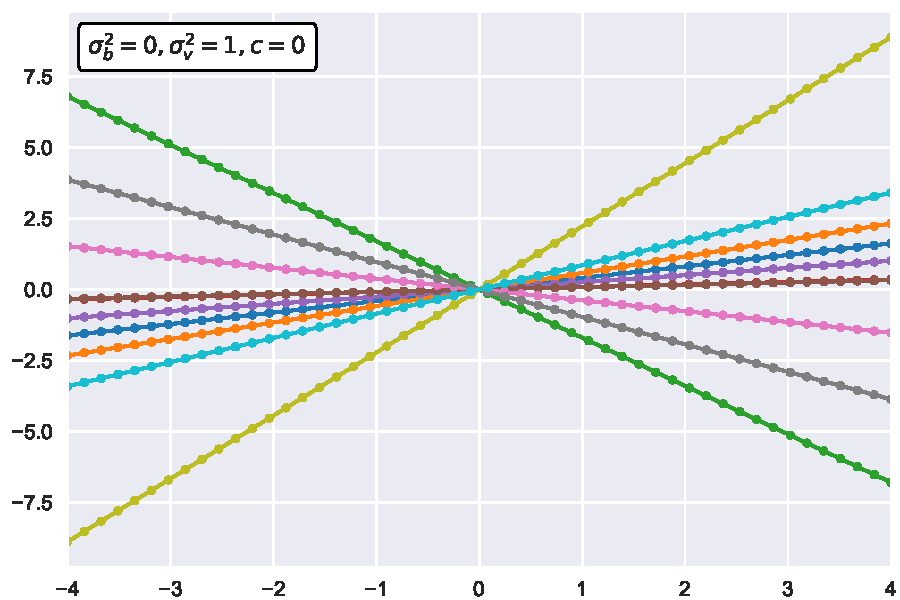
\includegraphics[width=\linewidth]{images/Gaussian process/Linear - sigmav=1.pdf}
  \caption{$\sigma_v^2=1$}
\end{subfigure}%
\begin{subfigure}{.5\textwidth}
  \centering
  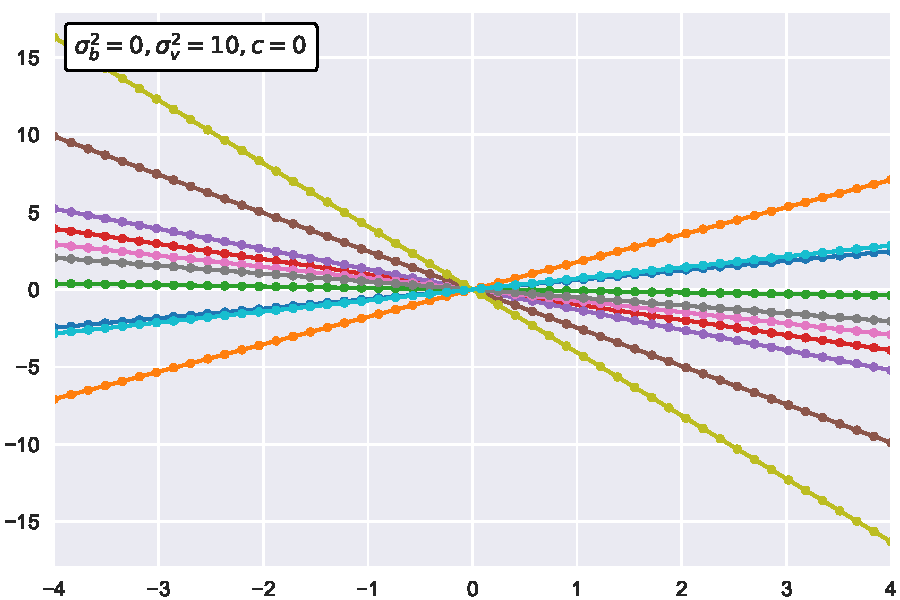
\includegraphics[width=\linewidth]{images/Gaussian process/Linear - sigmav=10.pdf}
  \caption{$\sigma_v^2=10$}
\end{subfigure}
\caption{Grafico di funzioni con distribuzione $f\sim \mathcal{GP}(\bm{0},k)$ dove $k(x,x')$ è il linear kernel e $\sigma_b^2=0$, $c=0$, il parametro $\sigma_v^2$ viene variato. Codice \ref{Linear - sigmav}.}
\label{10 sample linear modified sigmav}
\end{figure}

Dunque il parametro $\sigma_v^2$ influenza la pendenza delle rette, che è proporzionale al suo valore.

Per comprendere l'influenza della mean function, vengono di seguito mostrati grafici di funzioni con distribuzione $f\sim \mathcal{GP}(m,k)$ dove $m(x)=x^3$ e $k(\cdot,\cdot)$ è il linear kernel.


%%%%%%%%%%%%%%%%%%%%%%%%%%%%
%%%%%%%% IMMAGINE
%%%%%%%%%%%%%%%%%%%%%%%%%%%
\begin{figure}[h]
    \centering
    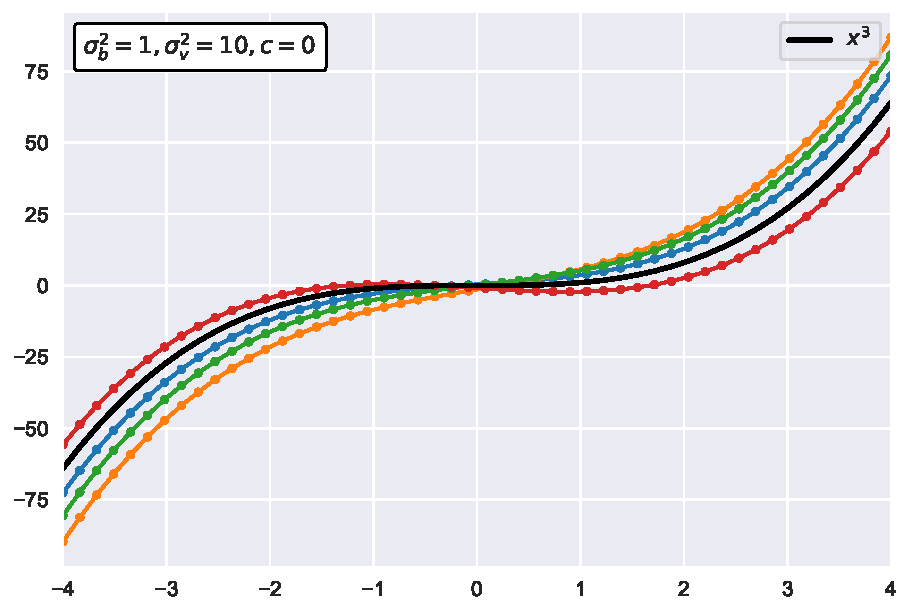
\includegraphics[width=0.85\textwidth]{images/Gaussian process/Linear - cubedmean.pdf}
    \caption{Grafico di funzioni con distribuzione $f\sim \mathcal{GP}(m,k)$ dove $m(x)=x^3$ e $k(x,x')$ è il linear kernel, $\sigma_b^2=1$, $\sigma_v^2=10$, $c=0$. Codice \ref{linear cubedmean}.}
    \label{10 sample linear kernel cubed mean}
\end{figure}


\newpage

Dal grafico è evidente che i grafici assomigliano alla funzione $x^3$. Sarà più chiaro nei prossimi esempi di kernel, ma dalla definizione di processo gaussiano (pensando alla distribuzione gaussiana multivariata, che generalizza) ogni punto è interpretabile come campione di una distribuzione gaussiana. Ricordando l'osservazione \ref{normal decomposition}, sappiamo che ogni distribuzione normale (univariata) è scomponibile in $Y=\mu+\sigma Z$ dove $Z\sim \mathcal{N}(0,1)$; dunque ogni punto $x_i$ del grafico di una funzione con distribuzione il processo gaussiano come in figura \ref{10 sample linear kernel cubed mean} ha scomposizione $x_i^3+k(x_i,x_i)Z$. È dunque chiaro dalla scomposizione di ogni punto che i grafici aggiungeranno alla funzione $x^3$ un addendo dovuto alla covariance function.





\subsection{Squared-exponential kernel}
%%%%%%%%%%%%%%%%
%%% SQUARED-EXPONENTIAL
%%%%%%%%%%%%%


%% A volte è usata ||x-x'||
\begin{defi}[Squared-exponential kernel]
Il \textbf{squared-exponential kernel} ha forma:
\[
k(x,x')=\sigma^2 \text{exp}\left( -\frac{(x-x')^2}{2l^2} \right).
\]
È dunque una covariance function isotropica.
\end{defi}

Viene riportato il grafico della funzione $k(x,x')$. Si noti che il parametro $\sigma^2$ influisce sul picco della funzione, mentre il parametro $l$ influisce indirettamente  modificandone la velocità con cui si annulla.



%%%%%%%%%%%%%%%%%%%%%%%%%
%%%%%%%%% IMMAGINE
%%%%%%%%%%%%%%%%%%%%%%%%
\begin{figure}[h]
    \centering
    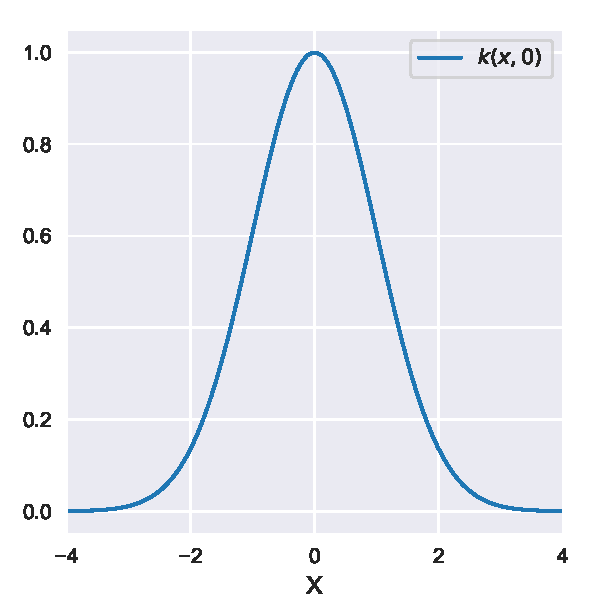
\includegraphics[width=0.6\textwidth]{images/Gaussian process/Squared-exponential kernel.pdf}
    \caption{Grafico di $k(x,x')$ squared-exponential kernel, $\sigma^2=1$ e $l^2=1$. Codice \ref{squared-exponential}.}
    \label{squared-exponential kernel}
\end{figure}

\newpage

Una funzione distribuita come il processo gaussiano con questo tipo di kernel è $C^\infty$. Esistono diverse variazioni di questo kernel codificanti ipotesi leggermente diverse
sulla continuità (anche locale) della funzione ma non sono negli interessi dell'elaborato. \footnote{Per approfondire si veda \cite{duvenaud_automatic_2014}}
\vspace{0.5cm}\\

Vengono di seguito mostrati grafici di funzioni con distribuzione $f\sim \mathcal{GP}(m,k)$ dove $m(x)=0$ e $k(x,x')$ è il squared-exponential kernel.


%%%%%%%%%%%%%%%%%%%%%%%%%
%%%%%%%%% IMMAGINE
%%%%%%%%%%%%%%%%%%%%%%%%
\begin{figure}[h]
    \centering
    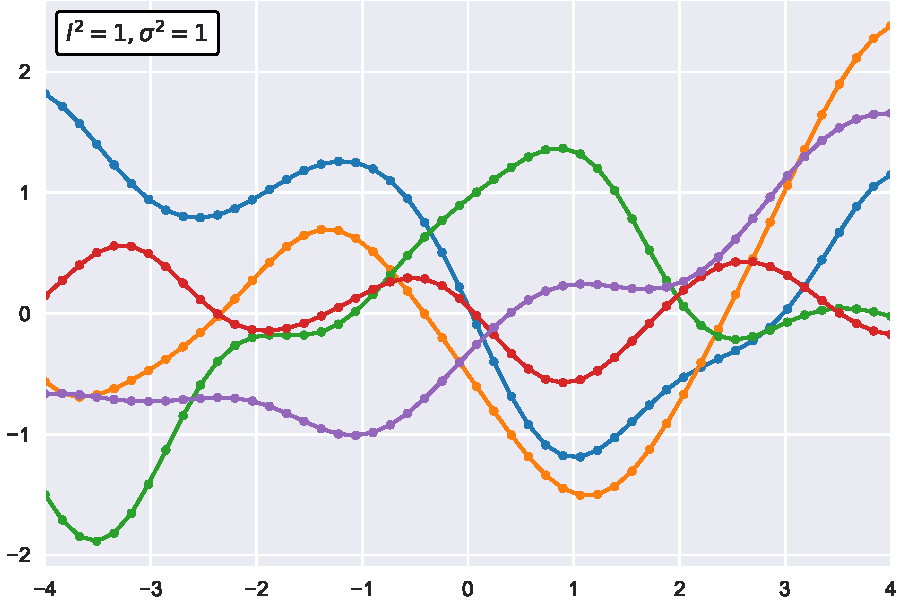
\includegraphics[width=0.85\textwidth]{images/Gaussian process/RBFSample.pdf}
    \caption{Grafico di funzioni con distribuzione $f\sim \mathcal{GP}(\bm{0},k)$ dove $k(x,x')$ è lo squared-exponential kernel e $l^2=1$, $\sigma^2=1$. Codice \ref{RBF sample}.}
    \label{10 sample exponential kerne zero mean}
\end{figure}

Dalla figura \ref{10 sample exponential kerne zero mean} è possibile notare la differenza che il kernel ha causato nella forma del grafico delle funzioni: paragonandolo alla figura \ref{10 sample linear kernel zero mean} risulta evidente l'importanza della scelta del kernel in funzione del contesto del suo utilizzo.\\
Come nel caso del linear kernel, imporre la mean function ad un'altra costante comporterà la traslazione delle funzioni sull'asse delle $y$.


\newpage 



Per comprendere l'influenza del parametro $\sigma^2$ vengono mostrati grafici di funzioni con distribuzione $f\sim \mathcal{GP}(m,k)$ dove $m(x)=0$ e $k(x,x')$ è il squared-exponential kernel, con $l^2=1$ e due valori diversi di $\sigma^2$.
%%%%%%%%%%%%%%%%%%%%%%%%%%%%%%%%%%%
%%%%%% IMMAGINI: PARAMETRO sigma
%%%%%%%%%%%%%%%%%%%%%%%%%%%%%%%%%%%
\begin{figure}[h]
\centering
\begin{subfigure}{.5\textwidth}
  \centering
  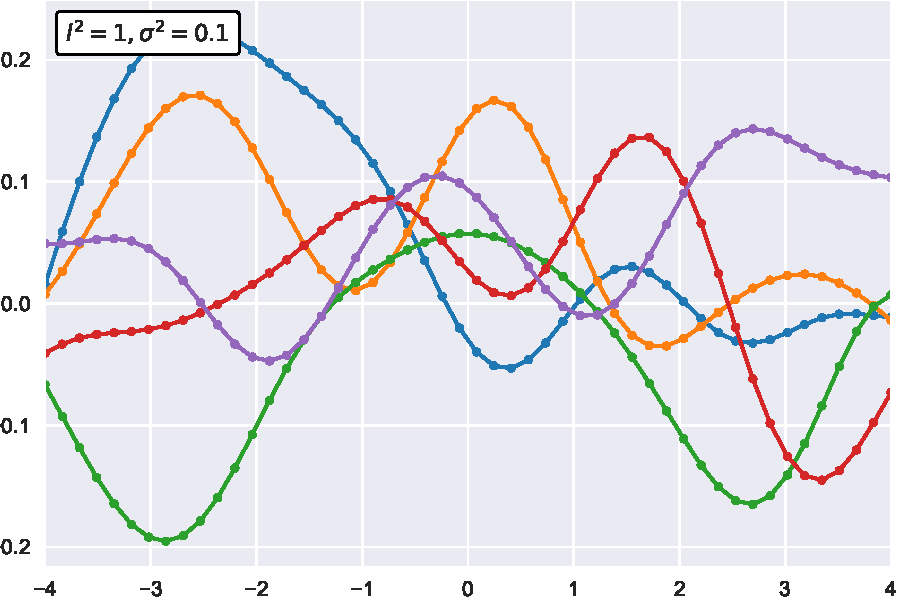
\includegraphics[width=\linewidth]{images/Gaussian process/RBF - sigma=01.pdf}
  \caption{$\sigma^2=0.1$}
\end{subfigure}%
\begin{subfigure}{.5\textwidth}
  \centering
  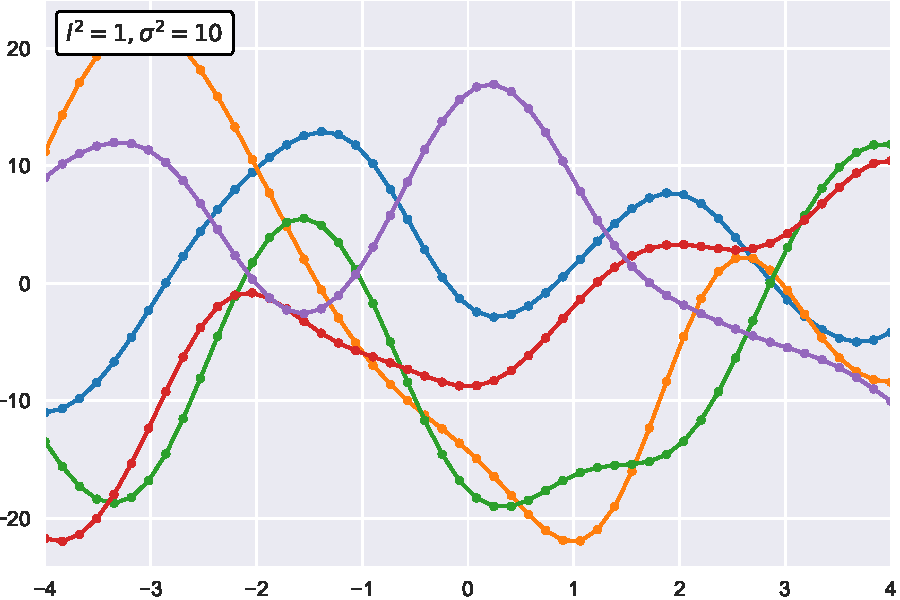
\includegraphics[width=\linewidth]{images/Gaussian process/RBF - sigma=10.pdf}
  \caption{$\sigma^2=10$}
\end{subfigure}
\caption{Grafico di funzioni con distribuzione $f\sim \mathcal{GP}(\bm{0},k)$ dove $k(x,x')$ è lo squared-exponential kernel e $l^2=1$, il parametro $\sigma^2$ viene variato. Codice \ref{RBF - sigma}.}
\label{10 sample exponential modified sigma}
\end{figure}

Nei due casi dunque cambia quanto le funzioni si distanziano dalla retta $x=0$, cioè proporzionalmente al valore di $\sigma^2$. In realtà $\sigma^2$ influisce sulla tendenza delle funzioni a distanziarsi dalla media $m(x)$.

Per comprendere l'influenza del parametro $l^2$, vengono di seguito mostrati grafici di funzioni con distribuzione $f\sim \mathcal{GP}(m,k)$ dove $m(x)=0$ e $k(x,x')$ è il squared-exponential kernel e il parametro $l^2$ viene variato.


%%%%%%%%%%%%%%%%%%%%%%%%%%%%%%%%%%%
%%%%%% IMMAGINI: PARAMETRO l
%%%%%%%%%%%%%%%%%%%%%%%%%%%%%%%%%%%
\begin{figure}[h]
\centering
\begin{subfigure}{.5\textwidth}
  \centering
  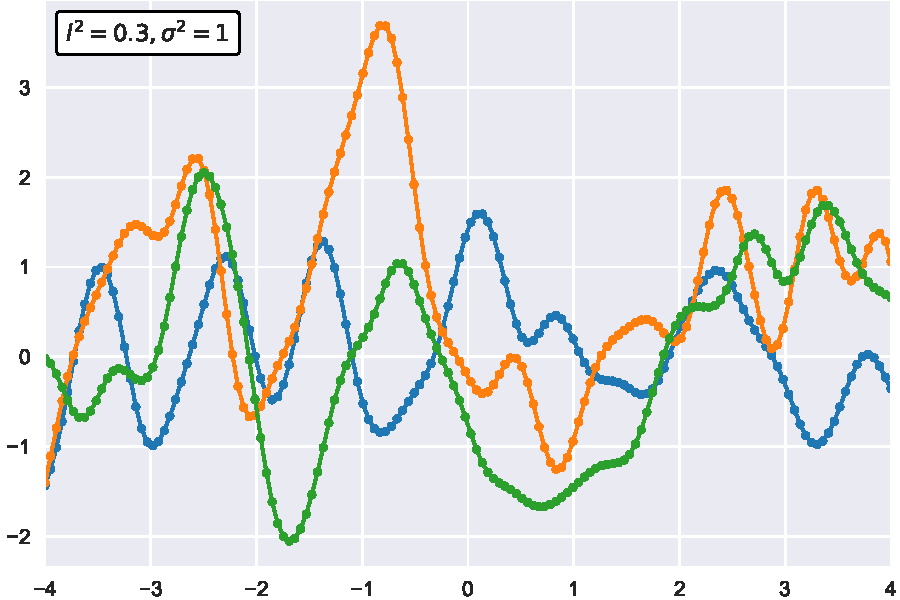
\includegraphics[width=\linewidth]{images/Gaussian process/RBF - l=03.pdf}
  \caption{$l^2=0.3$}
\end{subfigure}%
\begin{subfigure}{.5\textwidth}
  \centering
  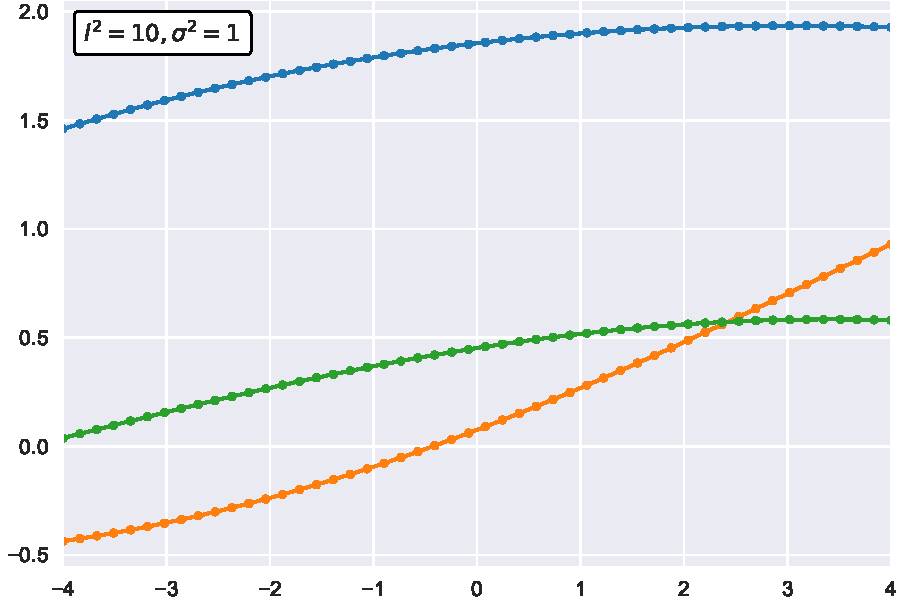
\includegraphics[width=\linewidth]{images/Gaussian process/RBF - l=10.pdf}
  \caption{$l^2=10$}
\end{subfigure}
\caption{Grafico di funzioni con distribuzione  $f\sim \mathcal{GP}(\bm{0},k)$ dove $k(x,x')$ è lo squared-exponential kernel e $\sigma^2=1$, il parametro $l^2$ viene variato. Codice \ref{codice9}.}
\label{10 sample exponential modified l}
\end{figure}

Il parametro $l^2$ dunque modifica la frequenza di oscillazione delle funzioni.

\newpage

Per comprendere l'influenza della mean function, vengono di seguito mostrati grafici di funzioni con distribuzione $f\sim \mathcal{GP}(m,k)$ dove $m(x)=x^3$ e $k(x,x')$ lo squared-exponential kernel.
%%%%%%%%%%%%%%%%%%%%%%%%%
%%%%%%%%% IMMAGINE
%%%%%%%%%%%%%%%%%%%%%%%%
\begin{figure}[h]
    \centering
    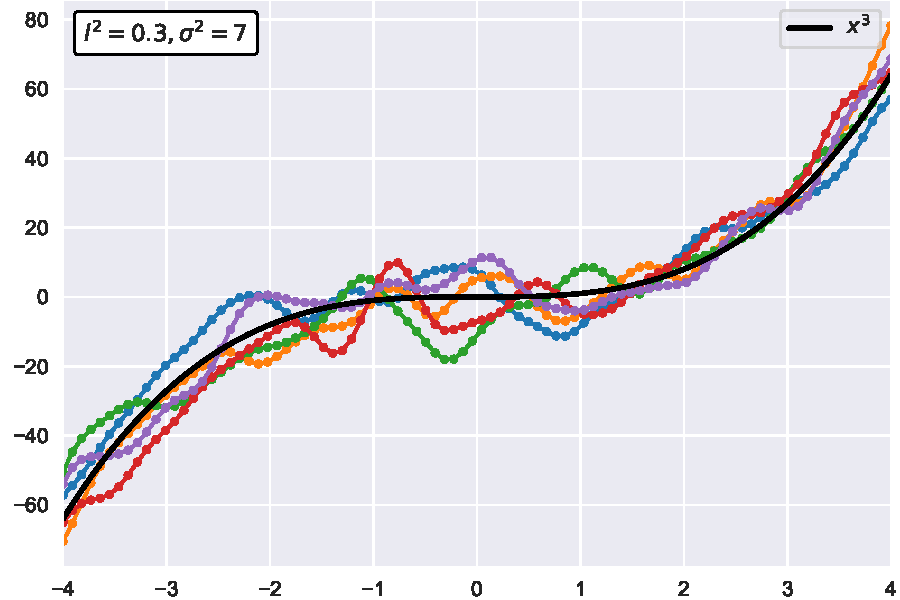
\includegraphics[width=0.85\textwidth]{images/Gaussian process/RBF - cubedmean.pdf}
    \caption{Grafico di funzioni con distribuzione  $f\sim \mathcal{GP}(m,k)$ dove $m(x)=x^3$ e $k(x,x')$ lo squared-exponential kernel, $\sigma^2=7$ e $l=0.3$. Codice \ref{codice10}.}
    \label{10 sample exponential kernel cubed mean}
\end{figure}

Sono stati scelti dei parametri in modo da risaltare i grafici delle funzioni. Con $\sigma^2=7$ (quindi un grande distanziamento dalla mean function) e $l^2=0.3$ (quindi una grande frequenza di oscillazione) le funzioni tendono a emulare la media $m(x)=x^3$ mantenendo le proprietà indotte dal kernel.

\newpage








\newpage

\subsection{Periodic kernel}

%%%%%%%%%%%%%%%%%%%%%%%%%%%%
%%%%%%%%% PERIODIC
%%%%%%%%%%%%%%%%%%%%%%%%%%%%
\begin{defi}[Periodic kernel]
Il \textbf{periodic kernel} ha forma:
\[
k(x,x')=\sigma^2 \text{exp}\left( -\frac{2}{l^2} \text{sin}^2\left( \pi \frac{|x-x'|}{p}\right)\right).
\]
Anche questo kernel è dunque isotropico.
\end{defi}

Viene riportato il grafico della funzione $k(x,x')$. Si noti che il parametro $\sigma^2$ influisce sul picco della funzione come nel \textit{squared-esponential kernel}, similmente il parametro $l^2$ influisce sulla funzione come nel precedente kernel, il parametro $p$ influenza la periodicità del kernel. 


%%%%%%%%%%%%%%%%%%%%%%%%%
%%%%%%%%% IMMAGINE
%%%%%%%%%%%%%%%%%%%%%%%%
\begin{figure}[h]
    \centering
    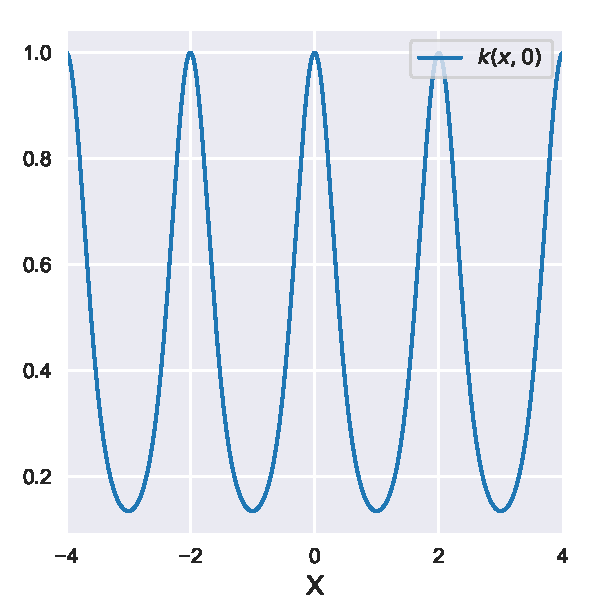
\includegraphics[width=0.6\textwidth]{images/Gaussian process/Periodic kernel.pdf}
    \caption{Grafico di $k(x,x')$ periodic kernel, $\sigma^2=1$, $l^2=1$, $p=2$. Codice \ref{periodic Kernel}.}
    \label{periodic kernel}
\end{figure}




\newpage
Vengono di seguito mostrati grafici di funzioni con distribuzione $f\sim \mathcal{GP}(m,k)$ dove $m(x)=0$ e $k(x,x')$ è il periodic kernel.

%%%%%%%%%%%%%%%%%%%%%%%%%
%%%%%%%%% IMMAGINE
%%%%%%%%%%%%%%%%%%%%%%%%
\begin{figure}[h]
    \centering
    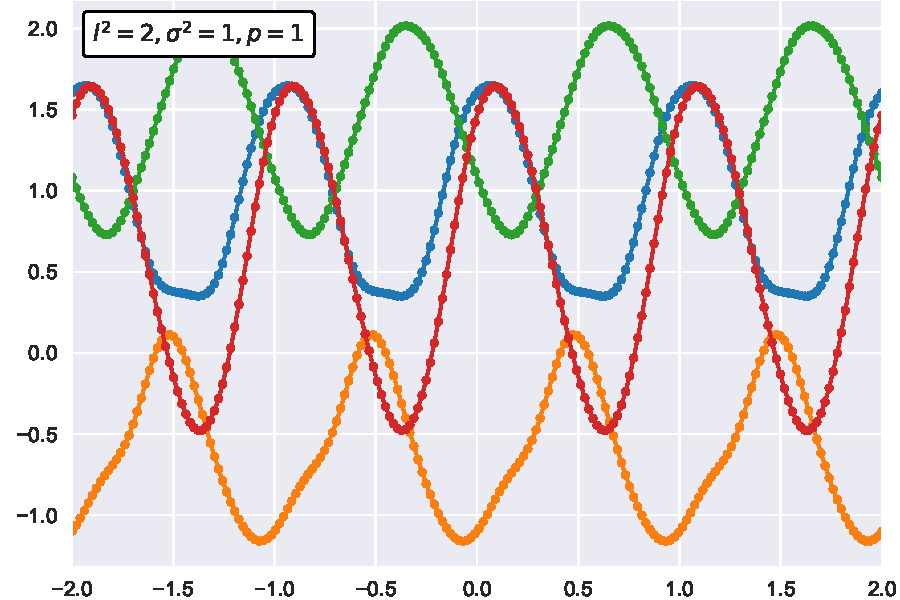
\includegraphics[width=0.85\textwidth]{images/Gaussian process/Periodic sample.pdf}
    \caption{Grafico di funzioni con distribuzione  $f\sim \mathcal{GP}(\bm{0},k)$ dove $k(x,x')$ è il periodic kernel e $\sigma^2=1$, $l^2=2$, $p=1$. Codice \ref{periodic sample}.}
    \label{3 sample periodic kerne zero mean}
\end{figure}

Come suggerisce il nome del kernel, le funzioni hanno andamento periodico.
Per comprendere l'influenza del parametro $\sigma^2$, vengono di seguito mostrati grafici di funzioni con distribuzione $f\sim \mathcal{GP}(m,k)$ dove $m(x)=0$ e $k(x,x')$ è il periodic kernel e il parametro $\sigma^2$ viene variato.

%%%%%%%%%%%%%%%%%%%%%%%%%%%%%%%%%%%
%%%%%% IMMAGINI: PARAMETRO sigma
%%%%%%%%%%%%%%%%%%%%%%%%%%%%%%%%%%%
\begin{figure}[h]
\centering
\begin{subfigure}{.5\textwidth}
  \centering
  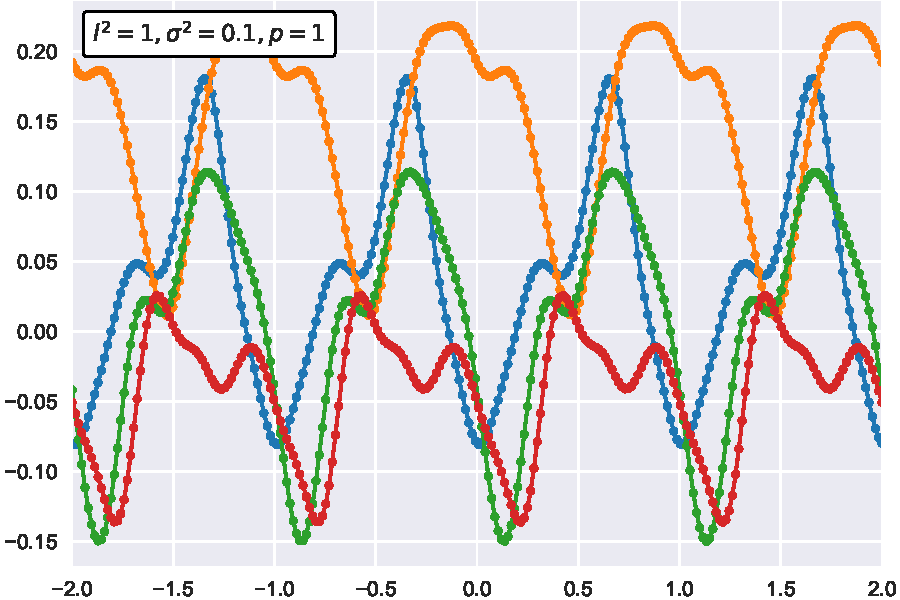
\includegraphics[width=\linewidth]{images/Gaussian process/Periodic - sigma=01.pdf}
  \caption{$\sigma^2=0.1$}
\end{subfigure}%
\begin{subfigure}{.5\textwidth}
  \centering
  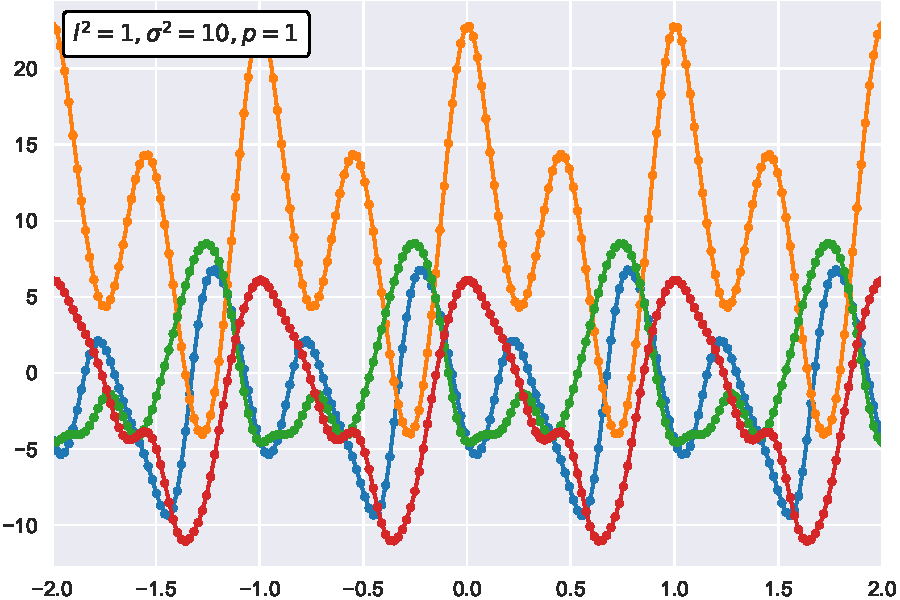
\includegraphics[width=\linewidth]{images/Gaussian process/Periodic - sigma=10.pdf}
  \caption{$\sigma^2=10$}
\end{subfigure}
\caption{Grafico di funzioni con distribuzione  $f\sim \mathcal{GP}(\bm{0},k)$ dove $k(x,x')$ è il periodic kernel e $l^2=1, p=1$, il parametro $\sigma^2$ viene variato. Codice \ref{Periodic sigma}.}
\label{10 sample periodic modified sigma}
\end{figure}

Il parametro $\sigma^2$ è dunque responsabile dell'allontamento delle funzioni dalla media, esattamente come per lo squared-exponential kernel (la figura \ref{10 sample exponential modified sigma} riporta infatti risultati simili).


\newpage

Per comprendere l'influenza del parametro $p$, vengono di seguito mostrati grafici di funzioni con distribuzione $f\sim \mathcal{GP}(m,k)$ dove $m(x)=0$ e $k(x,x')$ è il periodic kernel e il parametro $p$ viene variato.

%%%%%%%%%%%%%%%%%%%%%%%%%%%%%%%%%%%
%%%%%% IMMAGINI: PARAMETRO p
%%%%%%%%%%%%%%%%%%%%%%%%%%%%%%%%%%%
\begin{figure}[h]
\centering
\begin{subfigure}{.5\textwidth}
  \centering
  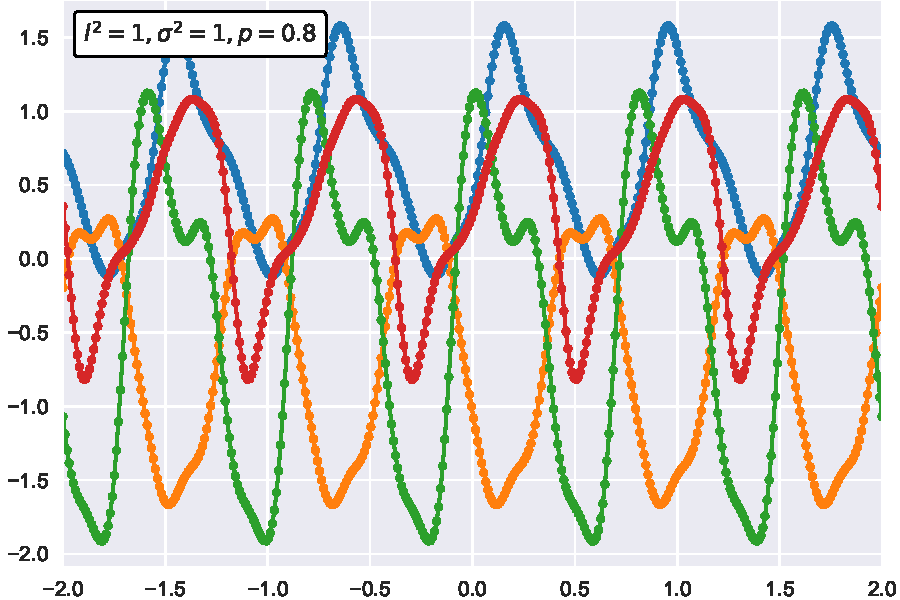
\includegraphics[width=\linewidth]{images/Gaussian process/Periodic - p=08.pdf}
  \caption{$p=0.8$}
\end{subfigure}%
\begin{subfigure}{.5\textwidth}
  \centering
  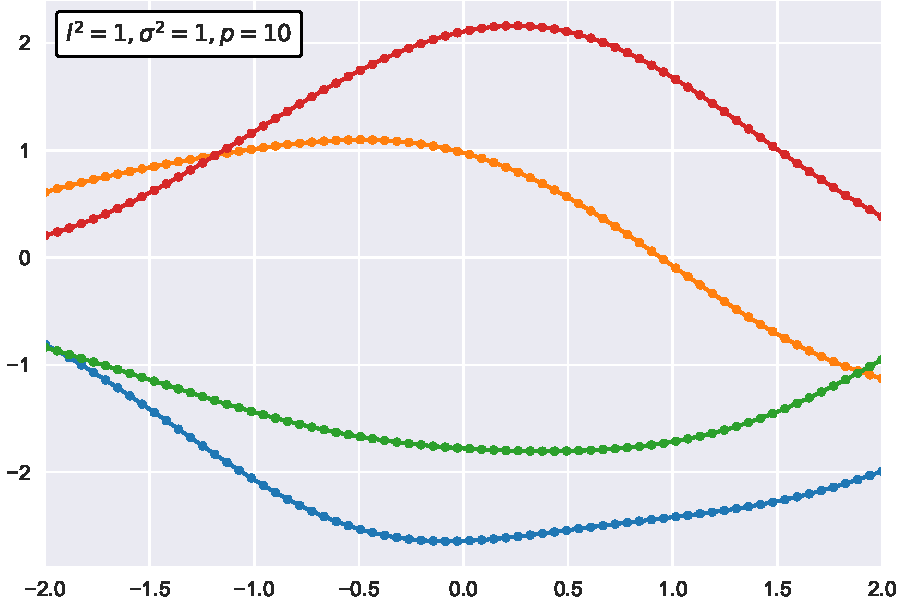
\includegraphics[width=\linewidth]{images/Gaussian process/Periodic - p=10.pdf}
  \caption{$p=10$}
\end{subfigure}
\caption{Grafico di funzioni con distribuzione  $f\sim \mathcal{GP}(\bm{0},k)$ dove $k(x,x')$ è il periodic kernel e $\sigma^2=1$, $l^2=1$ e il parametro $p$ viene variato. Codice \ref{periodic p}.}
\label{10 sample periodic modified p}
\end{figure}

Il parametro $p$ influenza dunque il periodo delle funzioni.

Per comprendere l'influenza del parametro $l^2$, vengono di seguito mostrati grafici di funzioni con distribuzione $f\sim \mathcal{GP}(m,k)$ dove $m(x)=0$ e $k(x,x')$ è il periodic kernel e il parametro $l^2$ viene variato.

%%%%%%%%%%%%%%%%%%%%%%%%%%%%%%%%%%%
%%%%%% IMMAGINI: PARAMETRO l
%%%%%%%%%%%%%%%%%%%%%%%%%%%%%%%%%%%
\begin{figure}[h]
\centering
\begin{subfigure}{.5\textwidth}
  \centering
  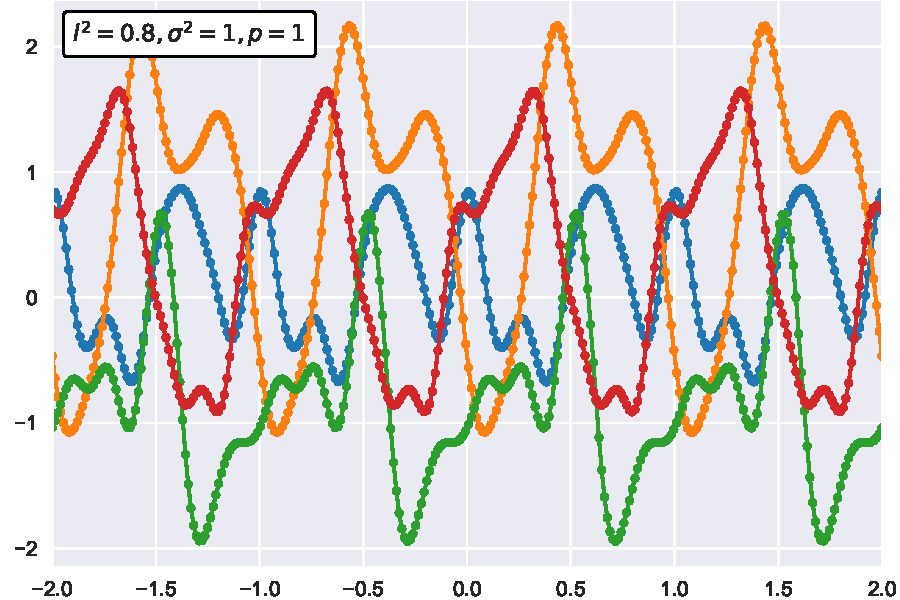
\includegraphics[width=\linewidth]{images/Gaussian process/Periodic - l=0.8.pdf}
  \caption{$l^2=0.8$}
\end{subfigure}%
\begin{subfigure}{.5\textwidth}
  \centering
  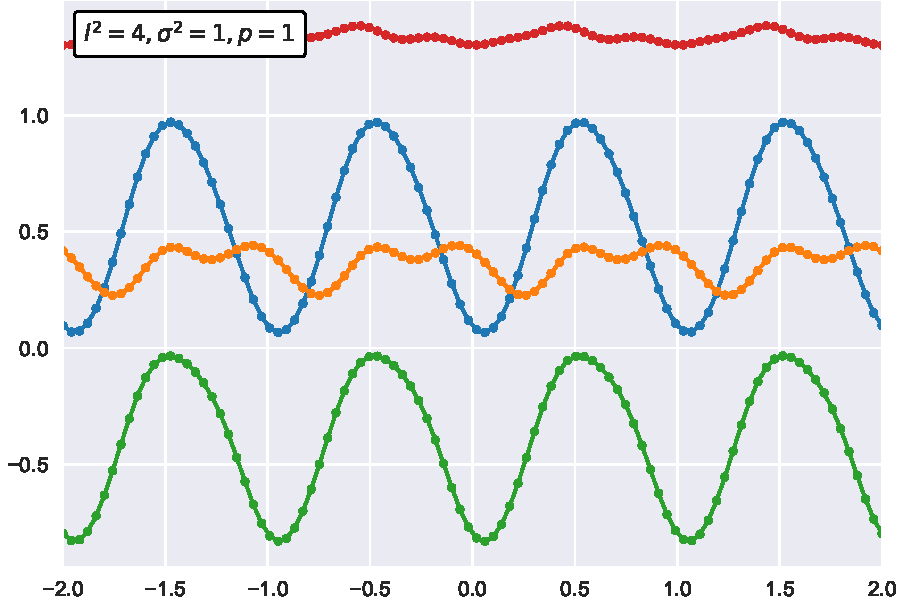
\includegraphics[width=\linewidth]{images/Gaussian process/Periodic - l=4.pdf}
  \caption{$l^2=4$}
\end{subfigure}
\caption{Grafico di funzioni con distribuzione  $f\sim \mathcal{GP}(\bm{0},k)$ dove $k(x,x')$ è il periodic kernel e $\sigma^2=1$, $p=1$ e il parametro $l^2$ viene variato. Codice \ref{periodic l}.}
\label{10 sample periodic modified l}
\end{figure}

Il parametro $l^2$ influenza dunque la "morbidezza" della frequenza delle funzioni.


\newpage 
Per comprendere l'influenza della mean function, vengono di seguito mostrati grafici di funzioni con distribuzione $f\sim \mathcal{GP}(m,k)$ dove $m(x)=x^3$ e $k(x,x')$ il periodic kernel.
%%%%%%%%%%%%%%%%%%%%%%%%%
%%%%%%%%% IMMAGINE
%%%%%%%%%%%%%%%%%%%%%%%%
\begin{figure}[h]
    \centering
    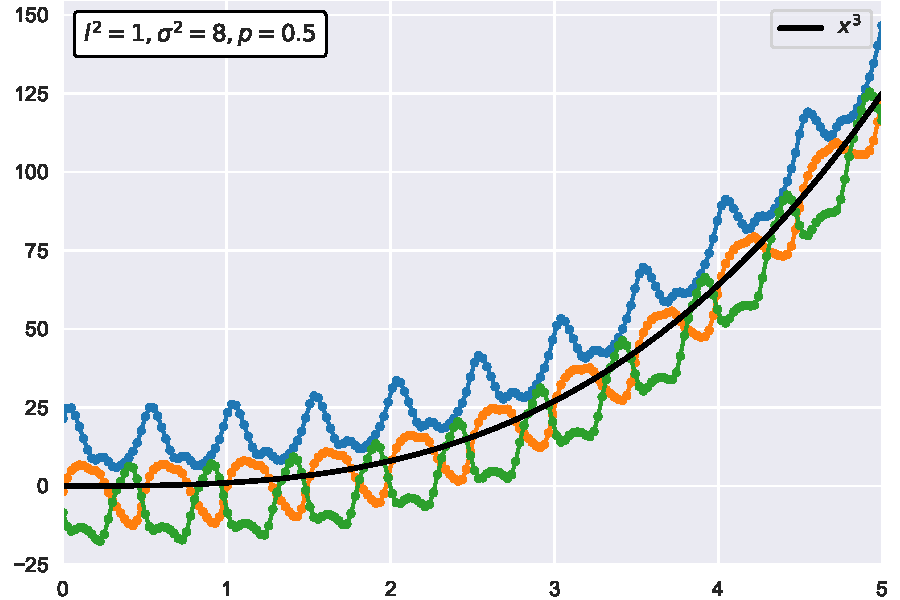
\includegraphics[width=0.85\textwidth]{images/Gaussian process/Periodic - cubedmean.pdf}
    \caption{Grafico di funzioni con distribuzione  $f\sim \mathcal{GP}(m,k)$ dove $m(x)=x^3$ e $k(x,x')$ il periodic kernel, $\sigma^2=8$, $l^2=1$ e $p=0.5$. Codice \ref{priodic cubedmean}.}
    \label{3 sample periodic kernel cubed mean}
\end{figure}

Sono stati scelti dei parametri in modo da risaltare i grafici delle funzioni. Con $\sigma^2=8$ (quindi un grande distanziamento dalla mean function) e $p=0.5$ (quindi una grande frequenza di oscillazione) e $l^2=1$ (quindi molto "spigolose") le funzioni tendono a emulare la media $m(x)=x^3$ mantenendo le proprietà indotte dal kernel.

\newpage



\subsection{Covariance function in più dimensioni}\label{multidimensionalKernel}
Si possono estendere le covariance function in più dimensioni in diversi modi. Poiché l'estensione a più dimensioni è pressocchè identica per ogni covariance function, viene mostrato il caso del squared-exponential kernel, in quanto verrà utilizzato nella parte di elaborato dedicata al training.\\
Per estendere il squared-exponential kernel è necessario estendere in più dimensioni la sottrazione $x-x'$. Il modo più semplice è considerare la norma $||x-x'||$, un modo più flessibile è considerare $(x-x')^\text{T}M(x-x')$ dove $M$ è una matrice.
In questo modo è possibile generalizzare il caso:
\[
k(x,x')=\sigma^2 \text{exp}\left( -\frac{||x-x'||^2}{2l^2} \right),
\]
che si può ottenere come:
\[
k(x,x')=\sigma^2 \text{exp}\left( -\frac{(x-x')^\text{T}M(x-x')}{2} \right)
\]
imponendo $M=l^{-2}I$.\\
La struttura del kernel con matrice permette di dotare ogni dimensione di una differente scala di lunghezza $l_i$, imponendo $M=\text{diag}(\bf{l})^{-2}$, dove $\mathbf{l}=(l_1,...,l_n)^\text{T}$. Questa caratteristica risulta fondamentale nel training (trattato successivamente nell'elaborato) perché se uno di questi $l_i$ diventa grande, la dimensione corrispondente (che si vedrà corrispondere ad un parametro da ottimizzare) "perde di rilevanza". L'immagine \ref{multidimensional} fornisce un esempio di un comportamento simile.

%%%%%%%%%%%%%%%%%%%%%%%%%
%%%%%%%%% IMMAGINE
%%%%%%%%%%%%%%%%%%%%%%%%
\begin{figure}[h]
    \centering
    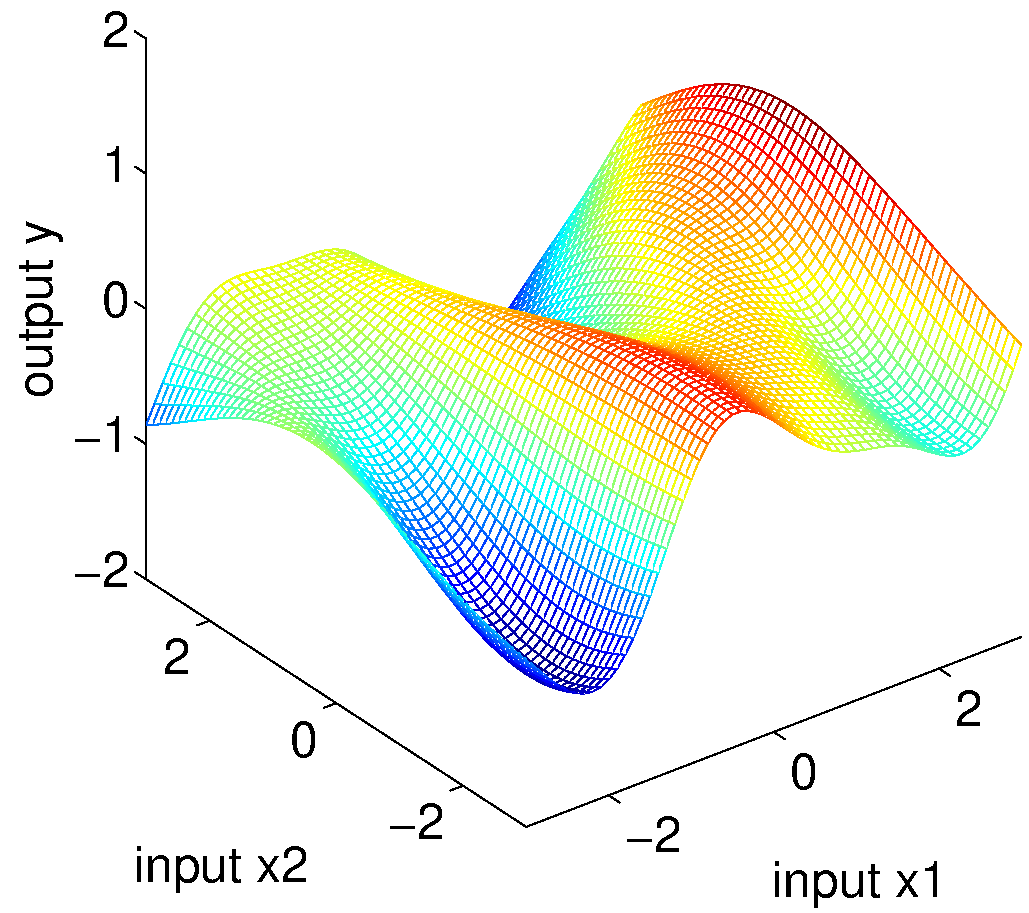
\includegraphics[width=0.6\textwidth]{images/Gaussian process/Multidimensional RBF.pdf}
    \caption{Grafico di funzione con distribuzione $f\sim \mathcal{GP}(0,k)$ con $k(x,x')$ lo squared-exponential kernel in due dimensioni in cui $M=\text{diag}(1,3)^{-2}$. La funzione tende a cambiare più velocemente lungo la direzione $x_1$ che lungo la direzione $x_2$. \cite{murphy_machine_2012}}
    \label{multidimensional}
\end{figure}




\newpage

\subsection{Combinare le covariance function}
Nelle precedenti sezioni è stata spiegata l'influenza della covariance function nella forma del grafico delle funzioni. Tuttavia non è raro dover usare funzioni con forme diverse da quelle imposte dalle covariance function precedentemente introdotte. In tal caso è possibile costruire un nuovo kernel secondo la proposizione \ref{combining kernel}.


\begin{prop} \label{combining kernel}
Dati due kernel $K_1(x,x')$ e $K_2(x,x')$, per le proprietà di un kernel i seguenti sono ancora kernel:
\[
\begin{array}{l}
    K(x,x') = c\cdot K_1(x,x') \quad \forall c>0 \text{ costante}\\
    K(x,x') = f(x)K_1(x,x')f(x') \quad \forall f \text{ funzione}\\
    K(x,x') = q(K_1(x,x')) \quad \forall q \text{ funz. polin. a coeff. non negativi}\\
    K(x,x') = \text{exp}(K_1(x,x'))\\
    K(x,x') = K_1(x,x')+K_2(x,x')\\
    K(x,x') = K_1(x,x')\times K_2(x,x')\\
\end{array}
\]
\end{prop}
Non è negli interessi dell'elaborato studiare a fondo le combinazioni possibili dei kernel introdotti; vengono però portati due semplici casi di combinazioni di kernel a titolo puramente illustrativo.

\newpage




\subsubsection{Squared exponential + periodic kernel}


%%%%%%%%%%%%%%%%%%%%%%%%%
%%%%%%%%% IMMAGINE
%%%%%%%%%%%%%%%%%%%%%%%%
\begin{figure}[h]
    \centering
    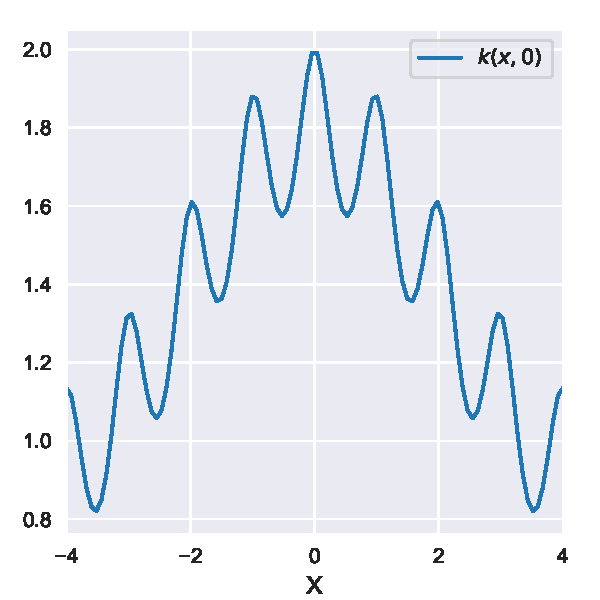
\includegraphics[width=0.55\textwidth]{images/Gaussian process/RBF + periodic kernel.pdf}
    \caption{Grafico di $k(x,x')$ squared-exponential kernel sommato a periodic kernel. $\sigma^2=1$, $l=2$, $p=1$. Codice \ref{RBF + periodic kernel}.}
    \label{SE + periodic kernel}
\end{figure}



%%%%%%%%%%%%%%%%%%%%%%%%%
%%%%%%%%% IMMAGINE
%%%%%%%%%%%%%%%%%%%%%%%%
\begin{figure}[h]
    \centering    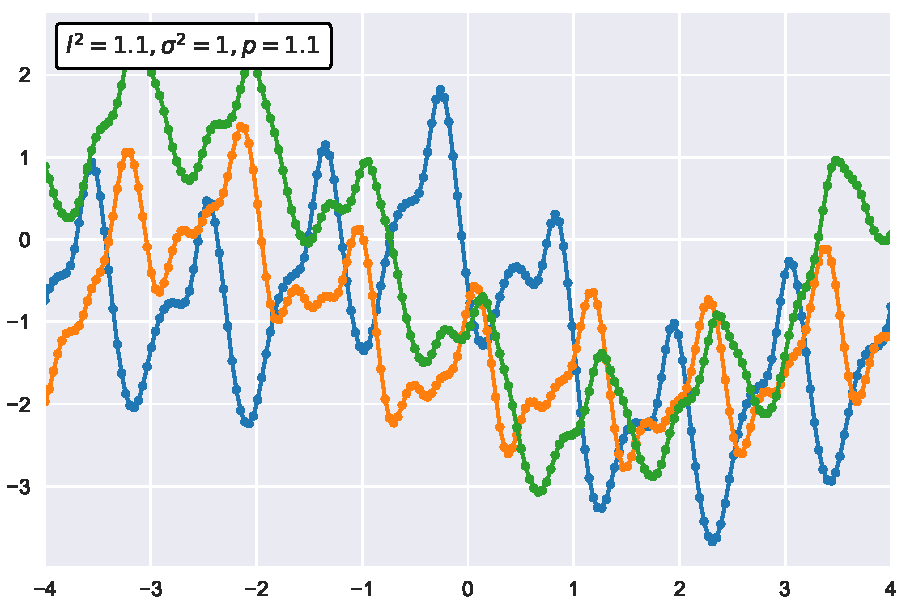
\includegraphics[width=0.69\textwidth]{images/Gaussian process/RBF + periodic sample.pdf}
    \caption{Grafico di funzioni con distribuzione  $f\sim \mathcal{GP}(\bm{0},k)$ dove $k(x,x')$ è lo squared-exponential sommato al periodic kernel e $l^2=1.1$, $\sigma^2=1$, $p=1.1$. Codice \ref{RBF + periodic sample}.}
    \label{SE + periodic sample}
\end{figure}

Combinare i due kernel genera dunque funzioni periodiche con delle perturbazioni sulla coppia degli assi.

\newpage

\subsubsection{Linear $\times$ linear kernel}

%%%%%%%%%%%%%%%%%%%%%%%%%
%%%%%%%%% IMMAGINE
%%%%%%%%%%%%%%%%%%%%%%%%
\begin{figure}[h]
    \centering
    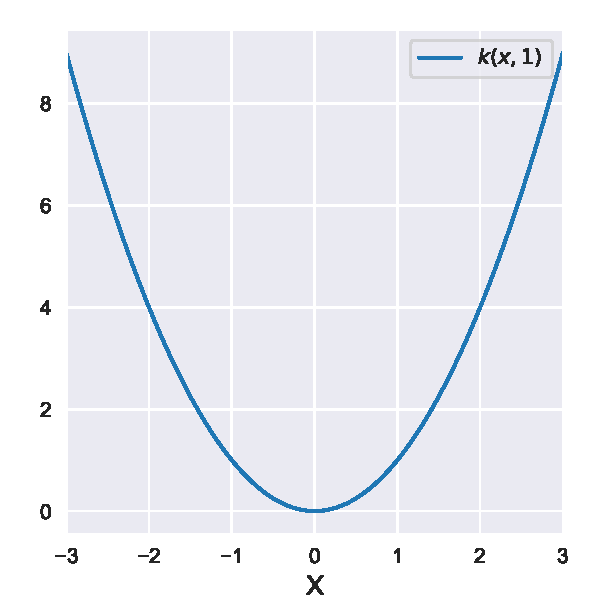
\includegraphics[width=0.55\textwidth]{images/Gaussian process/Linear x Linear kernel.pdf}
    \caption{Grafico di $k(x,x')$ linear kernel moltiplicato a linear kernel. $\sigma_b^2=0$, $\sigma_v^2=1$, $c=0$, $x'=1$. Codice \ref{linear x linear}.}
    \label{linear * linear kernel}
\end{figure}


%%%%%%%%%%%%%%%%%%%%%%%%%
%%%%%%%%% IMMAGINE
%%%%%%%%%%%%%%%%%%%%%%%%
\begin{figure}[h]
    \centering
    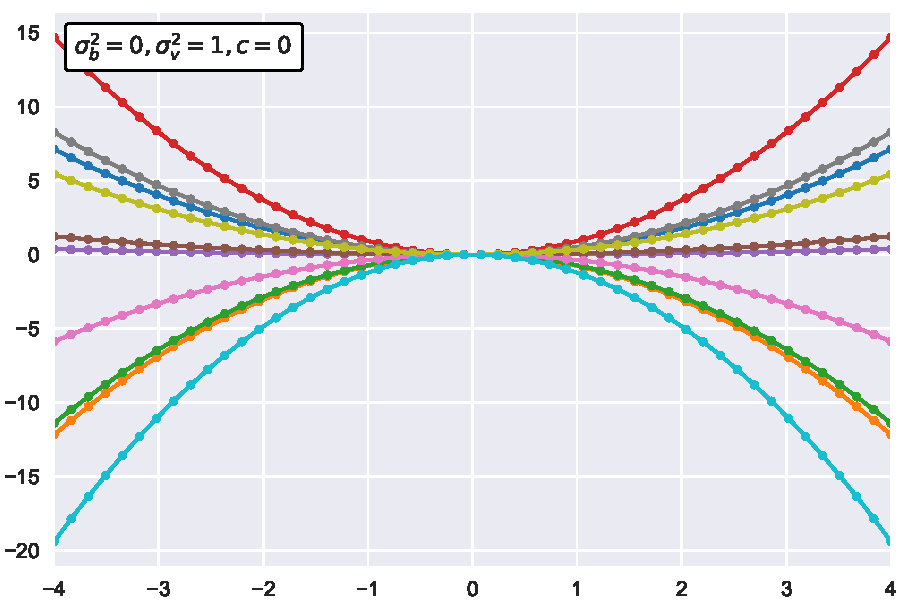
\includegraphics[width=0.68\textwidth]{images/Gaussian process/linear x linear sample.pdf}
    \caption{Grafico di funzioni con distribuzione  $f\sim \mathcal{GP}(\bm{0},k)$ dove $k(x,x')$ è il linear kernel moltiplicato al linear kernel e $\sigma_b^2=0$, $\sigma_v^2=1$, $c=0$. Codice \ref{linear x linear sample}.}
    \label{linear * linear sample}
\end{figure}


Combinare i due kernel genera dunque funzioni con comportamento parabolico. In un certo senso era possibile prevedere questo risultato ricordando che il linear kernel genera delle rette.

\newpage



\subsubsection{Esempio reale di covariance function composta}\label{section: mauna loa}
Viene ripreso da \cite{rasmussen_gaussian_2006} un esempio di regressione in cui è necessario comporre più kernel function.  I dati consistono in concentrazioni medie mensili di $CO_2$ atmosferica (in parti per milione di volume: $ppmv$) derivate da campioni d'aria raccolti presso l'osservatorio di Mauna Loa, nelle Hawaii, tra il 1958 e il 2003 (con alcuni valori mancanti). L'obiettivo è modellare la concentrazione di $CO_2$ in funzione del tempo $x$, cioè predire quella che è conosciuta come \textit{curva di Keeling}. Dalla figura \ref{CO2} sono evidenti alcune caratteristiche: una tendenza all'aumento a lungo termine, una pronunciata variazione stagionale e alcune irregolarità minori. 


%%%%%%%%%%%%%%%%%%%%%%%%%
%%%%%%%%% IMMAGINE
%%%%%%%%%%%%%%%%%%%%%%%%
\begin{figure}[ht]
    \centering
    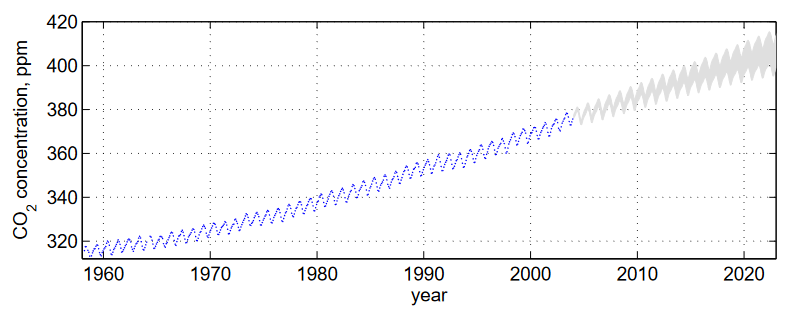
\includegraphics[width=1\textwidth]{images/Gaussian process/Co2_example.PNG}
    \caption{545 osservazioni delle medie mensili della concentrazione atmosferica di $CO_2$ tra il 1958 e il 2003, inoltre viene mostrata la regione di confidenza del $95\%$ per un modello di regressione di processo gaussiano a 20 anni nel futuro. \cite{rasmussen_gaussian_2006}}
    \label{CO2}
\end{figure}


Per modellare l'andamento regolare e crescente a lungo termine viene utilizzato uno squared-exponential kernel:
\[
k_1(x,x')=\theta_1^2\text{exp}\left(-\frac{(x-x')^2}{2\theta_2^2}\right).
\]


Viene usato il periodic kernel con un periodo di un anno per modellare la variazione stagionale. Poiché l'andamento stagionale non è esattamente periodico, viene considerato il prodotto con un squared-exponential kernel per consentire un decadimento non esattamente periodico: 
\[
k_2(x, x') = \theta^2_3 \text{exp}\left( - \frac{(x - x')^2}{2\theta^2_4} - \frac{2 \text{sin}^2(\pi(x - x'))}{\theta^2_5} \right).
\]
Per modellare le (piccole) irregolarità a medio termine viene utilizzato un \textit{rational quadratic} kernel (non è stato introdotto nell'elaborato): 
\[
k_3(x, x') = \theta^2_6 \left( 1 + \frac{(x - x')^2}{2\theta_8\theta^2_7} \right)^{-\theta_8}.
\] 
Infine, si modella il rumore come somma di un contributo di uno squared-exponential e di una componente indipendente:
\[
k_4(x_p, x_q) = \theta^2_9 \text{exp}\left( \frac{- (x_p - x_q)^2}{2\theta^2_{10}} \right) + \theta^2_{11} \delta_{pq}.
\]

Il kernel complessivo risulta:
\[
k(x,x')=k_1(x,x')+k_2(x,x')+k_3(x,x')+k_4(x,x'),
\]
dove si hanno $\bm{\theta}=(\theta_1,...,\theta_{11})$ iperparametri\footnote{Si veda \ref{gerarchica}.}. Dopo una fase di training del modello vengono dati dei valori ai $\theta_i$\footnote{Viene spiegato come questo venga fatto nel capitolo \ref{machineLearning}.}. La figura \ref{CO2} mostra come il modello predice l'andamento della concentrazione atmosferica di $CO_2$ nei venti anni successivi all'ultima misurazione, mostrando anche la regione di confidenza del novantacinque percento. Si nota che più si va avanti nel tempo e più la regione di confidenza si allarga.\\
Intuitivamente il modello sembra seguire bene l'andamento del grafico, seppur più avanti negli anni la regione di incertezza diventa più ampia, informando poco sull'effettiva concentrazione di $CO_2$. Nella figura \ref{CO2_comparison} viene comparata la predizione del modello con i dati reali presi dal sito del \href{https://gml.noaa.gov/ccgg/trends/}{Global Monitoring Laboratory}.


%%%%%%%%%%%%%%%%%%%%%%%%%
%%%%%%%%% IMMAGINE
%%%%%%%%%%%%%%%%%%%%%%%%
\begin{figure}[h]
    \centering
    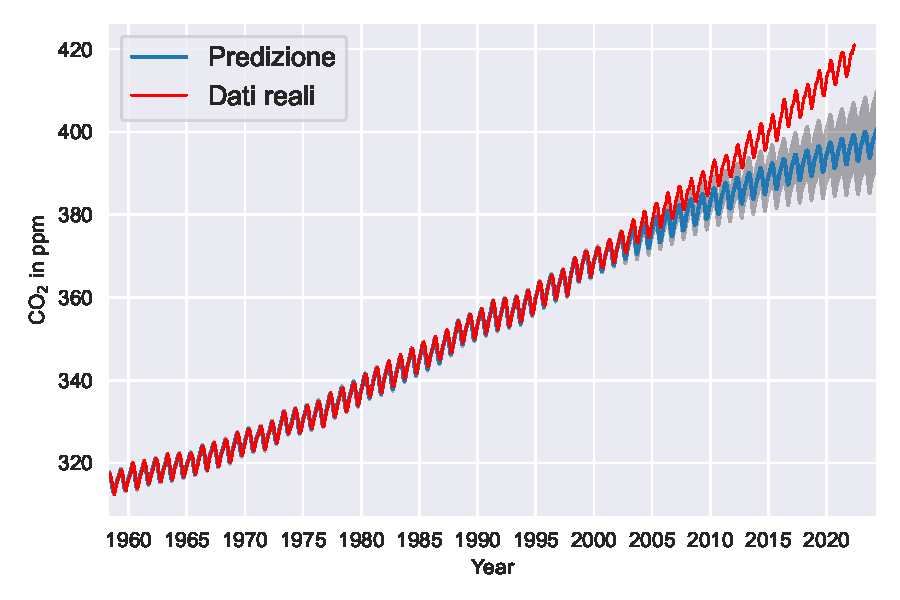
\includegraphics[width=1\textwidth]{images/Gaussian process/MaunaLoaPrediction.pdf}
    \caption{Comparazione della predizione della concentrazione di $CO_2$ con i dati reali fino a maggio 2022.}
    \label{CO2_comparison}
\end{figure}

\newpage

Si nota dunque che la previsione è stata conservativa nel lungo termine: il grande aumento nello concentrazione di $CO_2$ è dovuto, secondo alcune fonti, a come la flora ha risposto ai cambiamenti climatici (siccità e precipitazioni principalmente), ma anche alle grandi emissioni dovute all'uso di carburanti fossili.

In un certo senso, dunque, è ragionevole che la predizione non sia precisa negli ultimi anni poiché avrebbe dovuto prevedere eventi (dai cambiamenti climatici ai diversi tassi di consumo di carburante) che non erano presenti negli anni in cui il processo gaussiano "ha imparato".

In figura \ref{CO2_comparison_zoomed} viene ingrandita l'immagine precedente dal 1995 al 2022, dunque enfatizzando il periodo di tempo che il processo gaussiano ha predetto.

Si nota che dopo il 2003 la predizione è piuttosto imprecisa, non riuscendo a stare dietro ai veloci cambiamenti umani (in termini di inquinamento).  

%%%%%%%%%%%%%%%%%%%%%%%%%
%%%%%%%%% IMMAGINE
%%%%%%%%%%%%%%%%%%%%%%%%
\begin{figure}[h]
    \centering
    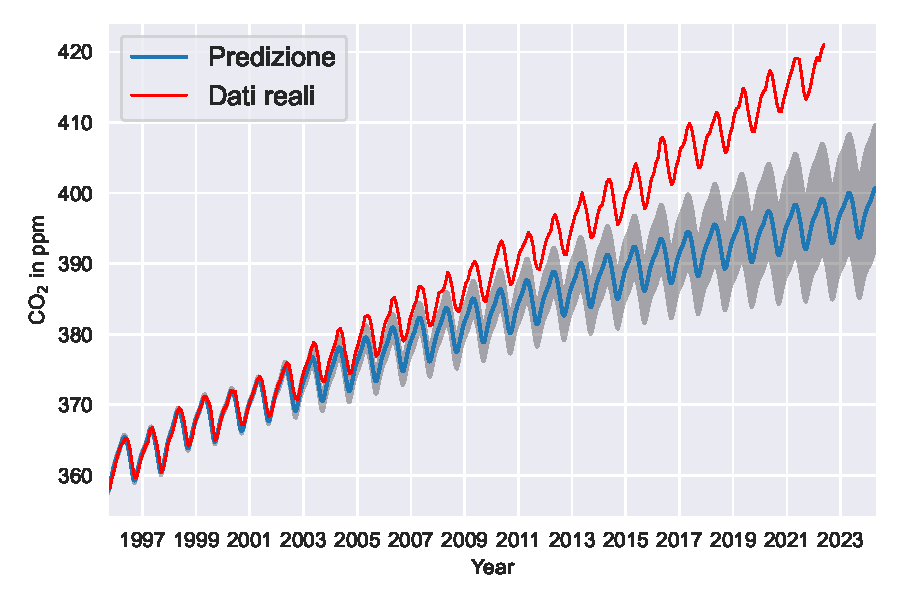
\includegraphics[width=1\textwidth]{images/Gaussian process/MaunaLoaPredictionZoom.pdf}
    \caption{Comparazione della predizione della concentrazione di $CO_2$ con i dati reali fino dal 1995 a maggio 2022.}
    \label{CO2_comparison_zoomed}
\end{figure}




\newpage



\section{Predizioni con osservazioni senza rumore}\label{regressioneGP}
In questa sezione viene spiegato come sfruttare le informazioni fornite dai \textit{training data} per generare una funzione che incorpori la conoscenza a priori nel caso di osservazioni senza rumore. \\


\begin{defi}[Noise-free training set]
Il \textbf{noise-free training set} è l'insieme di osservazioni \textit{noise-free} definito come: $\mathcal{D}=\{(x_n,y_n): n=1,...,N\}$ dove $y_n=f(x_n)$ è il valore osservato della funzione $f$ nel punto $x_n$. 
\end{defi}


Lo scopo del (noise-free) training set è quello di definire un insieme di punti $\mathcal{P}=\{x_n: n=1,...,N\}$ dei quali si conosce il valore della funzione per richiedere al processo gaussiano di generare funzioni che interpolino questo insieme di punti (dunque che abbiano valore $y_n$ su ogni $x_n\in \mathcal{P}$ senza incertezza).

\begin{defi}[Test set]
il \textbf{test set} è l'insieme di valori $X_*=\{x_n:n=1,...,N^*\}$ dei quali si vuole avere la predizione, cioè l'output della funzione.
\end{defi}

Pragmaticamente, quello che si sta facendo definendo il \textit{training set} $\mathcal{D}$ è aggiungere i punti di $\mathcal{P}$ all'insieme di punti su cui valutare la covariance function per costruire la matrice di covarianza\footnote{Come accennato in \ref{footnote 1}, per ottenere un grafico è necessario partire da un dominio finito. Per questo motivo si parla di \textit{matrice di covarianza}.}. Tramite il processo di condizionamento si ottiene la distribuzione \textit{a posteriori}, la distribuzione cioè delle funzioni che interpolano i punti del training set, come illustrato nella figura \ref{intuitiveExplanationOfConditioning}.


%%%%%%%%%%%%%%%%%%%%%%%%%
%%%%%%%%% IMMAGINE
%%%%%%%%%%%%%%%%%%%%%%%%
\begin{figure}[h]
    \centering
    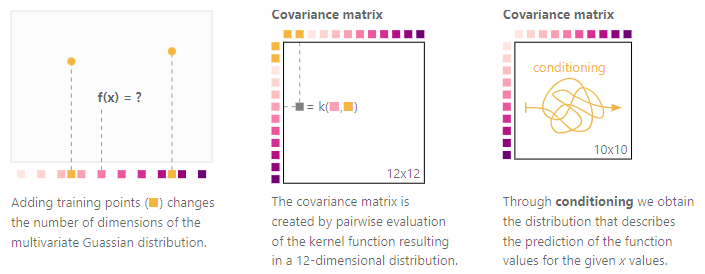
\includegraphics[width=1\textwidth]{images/Gaussian process/GPposterior.PNG}
    \caption{Spiegazione grafica di come viene incorporata la conoscenza a priori \cite{gortler_visual_2019}.}
    \label{intuitiveExplanationOfConditioning}
\end{figure}

\newpage
Si consideri ora una funzione distribuita come $f\sim \mathcal{GP}(m,k)$. 
Si consideri ora $X^*=\{x_i^*:i=1,\dots,N^*\}$ un \textit{test set} di cui si vuole predire gli output $\bm{f^*}=\left[f(x^*_1), \dots, f(x^*_{N^*}) \right]$; siano inoltre  $\bm{f}=\left[f(x_1), \dots, f(x_N) \right]$ gli output del training set dove $x_i\in \mathcal{P}$. Ricordando che gli output della funzione $f$ seguono una distribuzione gaussiana, è possibile ricavare la distribuzione congiunta:
\[
\begin{pmatrix}
\bm{f}\\
\bm{f^*}
\end{pmatrix}
=
\mathcal{N}\left(
\begin{pmatrix}
\bm{\mu}\\
\bm{\mu_*}
\end{pmatrix},
\begin{pmatrix}
\bm{K}_{X,X} & \bm{K}_{X,X^*}\\
\bm{K}_{X^*,X} & \bm{K}_{X^*,X^*}
\end{pmatrix}
\right)
\]

dove $\bm{\mu}=\begin{pmatrix}m(x_1) \\ \vdots \\ m(x_N)\end{pmatrix}$, $\bm{\mu_*}=\begin{pmatrix}m(x^*_1) \\ \vdots \\ m(x^*_{N^*})\end{pmatrix}$, $\bm{K}_{X,X}=k(X,X)$ è una matrice $N\times N$, $\bm{K}_{X,X^*}=k(X,X^*)$ è una matrice $N\times N^*$, $\bm{K}_{X^*,X}=k(X^*,X)$ è una matrice $N^*\times N$, $\bm{K}_{X^*,X^*}=k(X^*,X^*)$ è una matrice $N^*\times N^*$.\\

Dalla proposizione \ref{marginale-condizionata} ricaviamo la distribuzione condizionata di $\bm{f^*} | X^*, \mathcal{D}$:

\[
\bm{f^*} | X^*, \mathcal{D} \sim \mathcal{N}(\bm{\mu^*}, \bm{\Sigma^*})
\]

dove: 
\[
\begin{split}
\bm{\mu^*}=m(X^*)+\bm{K}_{X,X^*}^\text{T}\bm{K}^{-1}_{X,X}(\bm{f}-m(X))\\
\bm{\Sigma^*}=\bm{K}_{X^*,X^*}-\bm{K}_{X,X^*}^\text{T}\bm{K}^{-1}_{X,X}\bm{K}_{X,X^*}
\end{split}
\]


\newpage 
In figura \ref{Interpolation} viene mostrato un esempio grafico di interpolazione di sei punti.


%%%%%%%%%%%%%%%%%%%%%%%%%
%%%%%%%%% IMMAGINE
%%%%%%%%%%%%%%%%%%%%%%%%
\begin{figure}[h]
    \centering
    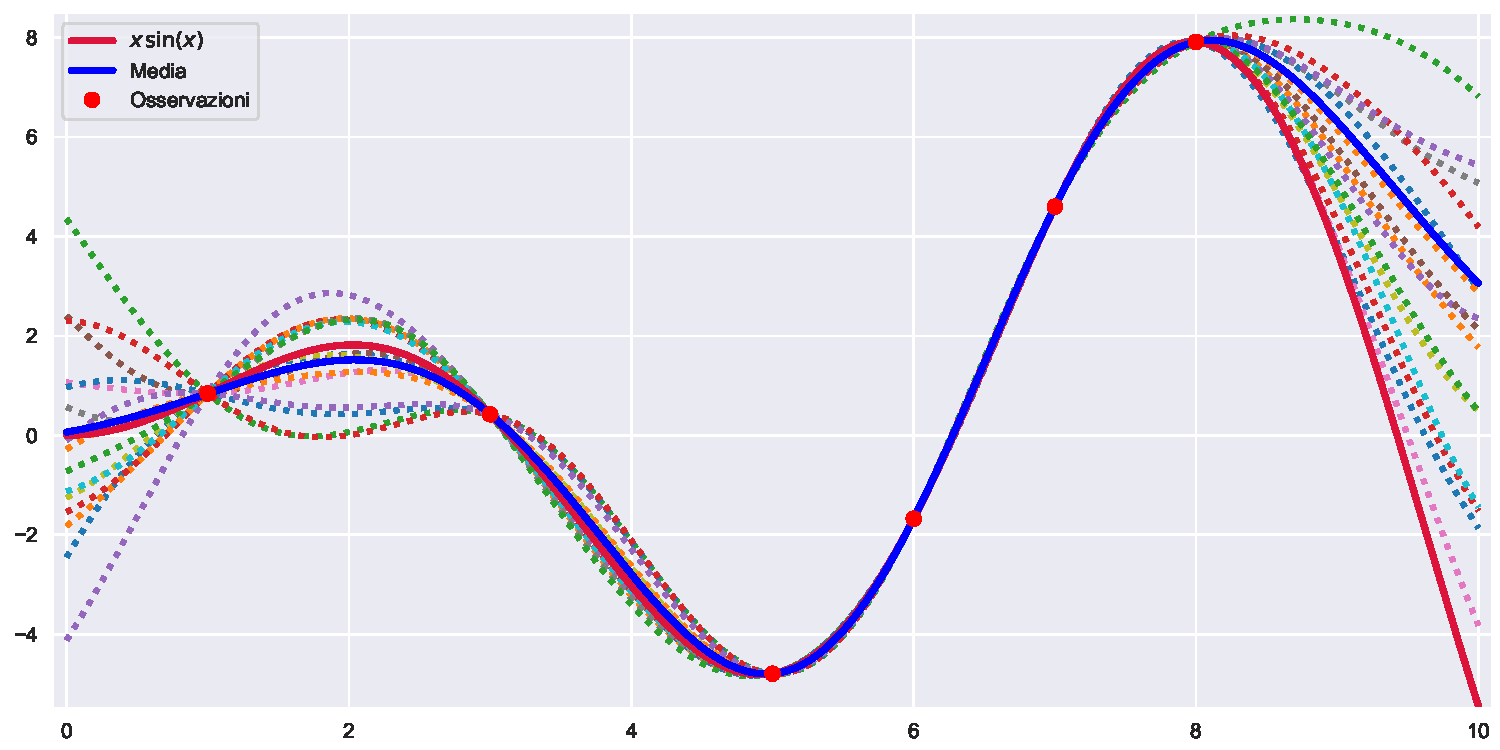
\includegraphics[width=1\textwidth]{images/Gaussian process/Noise-free - mean&f(x).pdf}
    \caption{Grafico di funzioni con distribuzione $f\sim \mathcal{GP}(\bm{0},k)$ dove $k(\cdot,\cdot)$ è il squared-exponential kernel; il processo gaussiano è stato condizionato per interpolare sei punti. Viene mostrata in rosso la funzione da cui sono stati scelti i punti da interpolare, in blu la media del processo gaussiano condizionato, come linee tratteggiate alcuni sample del processo gaussiano. Codice \ref{interpolation code}.}
    \label{Interpolation}
\end{figure}

La media del processo gaussiano condizionato per interpolare i sei punti è la più affidabile nel predire la funzione $x\cdot sin(x)$ da cui sono stati generati i punti da interpolare. Le funzioni con distribuzione il processo gaussiano condizionato hanno tutte la proprietà di interpolazione dei suddetti punti, tuttavia nel resto del piano si distanziano più facilmente dalla media, anche se tendono a restare nei suoi dintorni. Nella figura \ref{Interpolation confidence region} vengono sfruttate le informazioni della matrice di covarianza a posteriori per disegnare la regione di confidenza del 95\%, dentro la quale la maggior parte dei sample risiede.


\newpage
%%%%%%%%%%%%%%%%%%%%%%%%%
%%%%%%%%% IMMAGINE
%%%%%%%%%%%%%%%%%%%%%%%%
\begin{figure}[h]
    \centering
    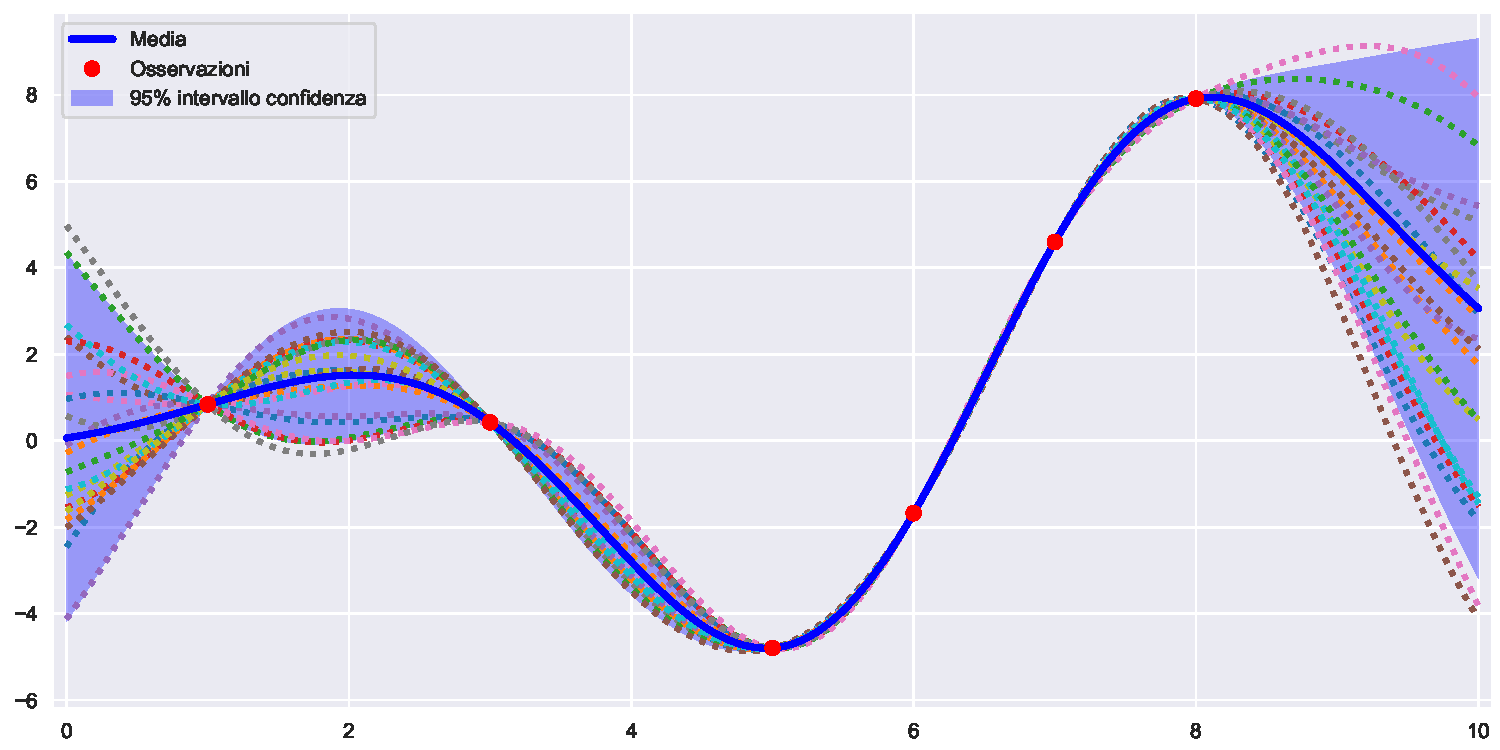
\includegraphics[width=1\textwidth]{images/Gaussian process/Noise-free - mean&samples.pdf}
    \caption{Grafico di funzioni con distribuzione $f\sim \mathcal{GP}(\bm{0},k)$ dove $k(\cdot,\cdot)$ è il squared-exponential kernel; il processo gaussiano è stato condizionato per interpolare sei punti. Viene mostrata in blu la regione di confidenza al 95\%, in blu la media del processo gaussiano condizionato e come linee tratteggiate alcuni sample. Codice \ref{interpolation confidence region code}.}
    \label{Interpolation confidence region}
\end{figure}

Come anticipato, all'interno dell'area data da $\bm{\mu^*}(x_i)\pm 1.96\bm{\Sigma^*}(x_i,x_i)$ (regione di confidenza al 95\%) risiedono la maggior parte dei sample della distribuzione a posteriori. Più ci si distanzia dai punti interpolati e più facilmente le funzioni si discostano dalla media, tendendo ad uscire dall'area di incertezza, come si osserva ad esempio nella zona nei pressi di $x=10$ della figura \ref{Interpolation confidence region}.



\section{Predizioni con osservazioni rumorose}\label{noisyPrediction}
In questa sezione viene spiegato come sfruttare le informazioni fornite dai \textit{training data} per generare una funzione che incorpori la conoscenza a priori nel caso di osservazioni con rumore. \\

\begin{defi}[Noisy training set]
Il \textbf{noisy training set} è l'insieme di osservazioni \textit{noisy} (cioè con una componente di errore) definito come: $\mathcal{D}=\{(x_n,y_n): n=1,...,N\}$ dove $y_n=f(x_n)+\epsilon$ è il valore osservato della funzione $f$ nel punto $x_n$ con una componente di rumore $\epsilon\sim \mathcal{N}(0,\sigma_n^2)$ indipendente e identicamente distribuito. 
\end{defi}
In questo caso si ha:
\[
\text{Cov}(y_p,y_q)=k(x_p,x_q)+\sigma_n^2 \delta_{pq},
\]
o equivalentemente:
\[
\text{Cov}(\mathbf{y})=k(X,X)+\sigma_n^2I.
\]

\newpage

Viene usata una notazione analoga alla sezione \ref{regressioneGP}: $X^*=\{x_i^*:i=1,\dots,N^*\}$ è il \textit{test set} di cui si vogliono predire gli output $\bm{f^*}=\left[f(x^*_1), \dots, f(x^*_{N^*}) \right]$;  $\bm{y}=\left[f(x_1)+\epsilon, \dots, f(x_N)+\epsilon \right]$ gli output del training set. \\
Si procede come nel caso della predizione con osservazioni senza rumore:
\[
\begin{pmatrix}
\bm{y}\\
\bm{f^*}
\end{pmatrix}
=
\mathcal{N}\left(
\begin{pmatrix}
\bm{\mu}\\
\bm{\mu_*}
\end{pmatrix},
\begin{pmatrix}
\bm{K}_{X,X}+\sigma_n^2I & \bm{K}_{X,X^*}\\
\bm{K}_{X^*,X} & \bm{K}_{X^*,X^*}
\end{pmatrix}
\right)
\]
Si ricava:
\[
\bm{f^*} | X^*, \mathcal{D} \sim \mathcal{N}(\bm{\mu^*}, \bm{\Sigma^*})
\]

dove: 
\[
\begin{split}
\bm{\mu^*}=m(X^*)+\bm{K}_{X,X^*}^\text{T}(\bm{K}_{X,X}+\sigma_n^2I)^{-1}(\bm{y}-m(X))\\
\bm{\Sigma^*}=\bm{K}_{X^*,X^*}-\bm{K}_{X,X^*}^\text{T}(\bm{K}_{X,X}+\sigma_n^2I)^{-1}\bm{K}_{X,X^*}
\end{split}
\]


In figura \ref{Noisy} viene mostrato un esempio grafico di come un processo gaussiano interpreti le informazioni date da osservazioni con rumore per predire una funzione.
Come ci si può aspettare, essendo le osservazioni in questo caso con rumore, il processo gaussiano ha bisogno di più osservazioni per poter predire l'andamento della funzione. Non verificandosi interpolazione, il processo gaussiano predice la funzione con minore precisione.
%%%%%%%%%%%%%%%%%%%%%%%%%
%%%%%%%%% IMMAGINE
%%%%%%%%%%%%%%%%%%%%%%%%
\begin{figure}[h]
    \centering
    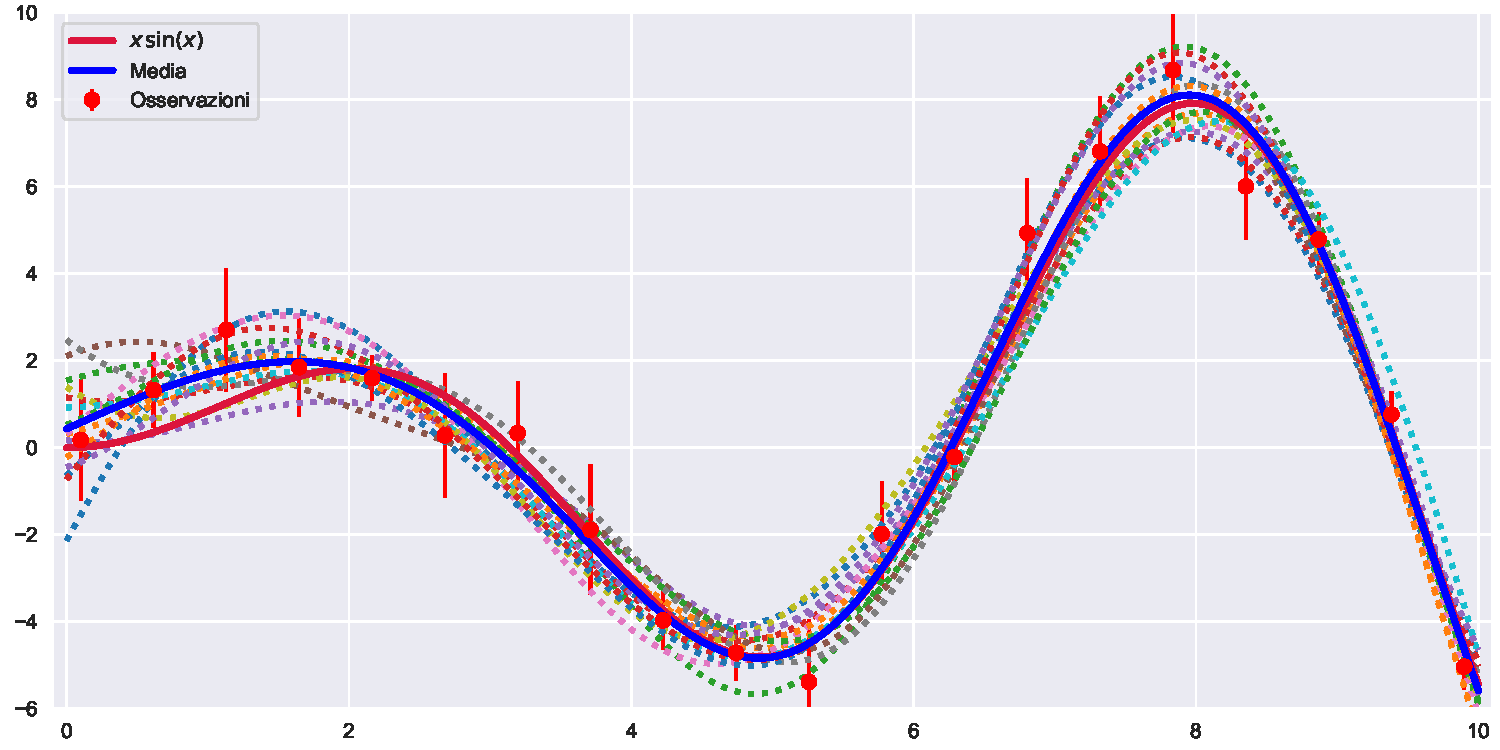
\includegraphics[width=1\textwidth]{images/Gaussian process/Noise - mean&f(x).pdf}
    \caption{Grafico di funzioni con distribuzione $f\sim \mathcal{GP}(\bm{0},k)$ dove $k(\cdot,\cdot)$ è il squared-exponential kernel; il processo gaussiano è stato condizionato per predire una funzione a partire dalle sue osservazioni rumorose. Viene mostrata in rosso la funzione da predire, in rosso i punti osservati della funzione con le barre rappresentanti il rumore, in blu la media del processo gaussiano condizionato, come linee tratteggiate alcuni sample del processo gaussiano. Codice \ref{Noise code}.}
    \label{Noisy}
\end{figure}

\newpage

Anche in questo caso la media del processo gaussiano condizionato rappresenta la funzione che meglio predice $x\cdot sin(x)$. Poiché le osservazioni presentano un errore, non si ha interpolazione dei punti seppur, tendenzialmente, la media e i sample del processo gaussiano tocchino almeno le barre di errore di ogni punto.
Sono stati presi in considerazione più punti del caso noise-free poiché con meno punti non si sarebbe ottenuto un risultato così "preciso" (comunque con un comportamento diverso da quello con osservazioni senza rumore).

Se nel caso senza rumore i sample tendenvano a rimanere nei pressi della media nelle vicinanze di ogni punto interpolato, qui la vicinanza alla media dipende sia dai punti che dal loro errore: nei pressi di punti con minore rumore (cioè con barre più corte) le funzioni tendono ad avvicinarsi alla media. Viceversa, nei pressi di funzioni con un grande errore (barre più lunghe) le funzioni tendono ad allontanarsi con più facilità dalla media.

Anche in questo caso è possibile disegnare la regione di confidenza del 95\%. La regione di confidenza ha ampiezza proporzionale alla lunghezza delle barre delle osservazioni; di conseguenza la regione di confidenza ha comportamento decisamente diverso dal caso noise-free.

%%%%%%%%%%%%%%%%%%%%%%%%%
%%%%%%%%% IMMAGINE
%%%%%%%%%%%%%%%%%%%%%%%%
\begin{figure}[h]
    \centering
    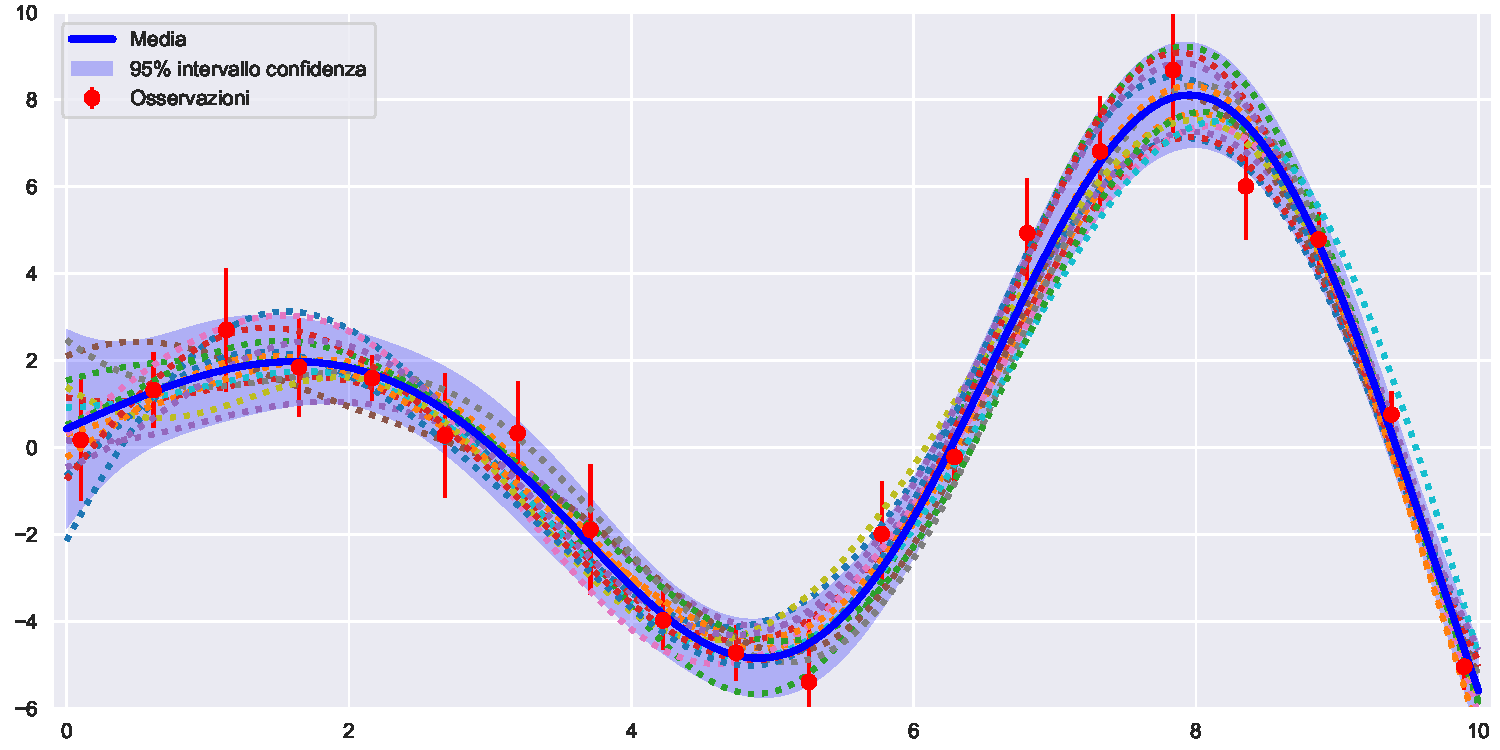
\includegraphics[width=1\textwidth]{images/Gaussian process/Noise - mean&samples.pdf}
    \caption{Grafico di funzioni con distribuzione $f\sim \mathcal{GP}(\bm{0},k)$ dove $k(\cdot,\cdot)$ è il squared-exponential kernel; il processo gaussiano è stato condizionato per predire una funzione a partire dalle sue osservazioni rumorose. Viene mostrata in blu la regione di confidenza al 95\%, in rosso con le barre di errore le osservazioni, in blu la media del processo gaussiano condizionato e come linee tratteggiate alcuni sample. Codice \ref{Noise confidence region code}.}
    \label{Noisy confidence region}
\end{figure}